\documentclass[a4paper, 11pt]{article}

\usepackage[utf8]{inputenc}
\usepackage[T1]{fontenc}
\usepackage[italian]{babel}
\usepackage{amsmath}
\usepackage{amsthm}
\usepackage{amssymb}
\usepackage{geometry}
\usepackage[hidelinks]{hyperref}
\usepackage{graphicx}
\usepackage{booktabs}
\usepackage{enumitem} 
\usepackage{parskip}
\usepackage[most]{tcolorbox}
\usepackage{booktabs}
\usepackage{tabularx}

\geometry{a4paper, margin=2cm}

\newenvironment{example}[1][]{
  \par\noindent\textbf{Esempio%
  \if\relax\detokenize{#1}\relax\else\ (\textbf{#1})\fi.}\ }{}

\newenvironment{definition}[1][]{
  \par\noindent\textbf{Definizione%
  \if\relax\detokenize{#1}\relax\else\ (\textbf{#1})\fi.}\ }{}

\newtheorem{theorem}{Teorema}

\title{Appunti S.I. da 3 CFU}
\author{Ionut Georgian Zbirciog}
\begin{document}

\maketitle

\tableofcontents
\newpage

\section{Gruppi}

\begin{definition}
    Un gruppo $(\mathbb{G}, \star)$ è una struttura algebrica composta da un insieme di elementi $\mathbb{G}$ e un'operazione $\star$. Per essere definito tale, deve soddisfare quattro proprietà fondamentali:
    \begin{description}
        \item[Chiusura:] Per ogni coppia di elementi $a,\ b \in \mathbb{G}$, il risultato $a \star b \in \mathbb{G}$.
        \item[Identità (Elemento Neutro):] Esiste un elemento $I$, tale che, per ogni $a \in \mathbb{G}$, si ha che $a \star I = I \star a = a$.
        \item[Inverso:] Per ogni elemento $a \in \mathbb{G}$, esiste un elemento $a^{-1} \in \mathbb{G}$ tale che $a \star a^{-1} = I$.
        \item[Associatività:] Per ogni $a,\ b,\ c \in \mathbb{G}$, vale che $(a \star b) \star c = a \star (b \star c)$.  
    \end{description}
\end{definition}

Inoltre, diremo che il gruppo è \textbf{Abeliano} se vale anche la proprietà \textbf{commutativa}, ossia $a\ \star\ b = b\ \star\ a$.

\subsection{Il Gruppo $\mathbb{Z}_p^*$}

Il gruppo $\mathbb{Z}_p^* = (\mathbb{Z}_p, \cdot)$ è il gruppo moltiplicativo modulo un numero primo $p$. È un gruppo finito composto da $p-1$ elementi:
\[
    \mathbb{Z}_p^* = \{1, 2, \dots, p - 1\}
\]
L'unica operazione considerata è \textbf{moltiplicazione modulo} $p$; la somma viene esclusa, altrimenti si parlerebbe di un campo $\mathbb{F}_p$.
 
In generale un elemento $x$ ha un inverso modulo $N$ se e solo se $gcd(x, N) = 1$. Poiché $p$ è primo, tutti gli elementi da $1$ a $p - 1$ hanno un inverso. Per gruppi molto grandi, l'inverso si calcola con l'\textbf{Algoritmo Euclideo Esteso}.

Lo zero non fa parte del gruppo perché non ammette inverso moltiplicativo.

\begin{example}
    Consideriamo il gruppo $\mathbb{Z}_{11}^* = \{1, 2, 3, 4, 5, 6, 7, 8, 9, 10\}$.
    Gli inversi degli elementi sono:

    \begin{align*}
        & 1 \to 1; \\
        & 2 \to 6; \text{ infatti } 2 \cdot 6 \mod 11 = 12 \mod 11 = 1. \\
        & 3 \to 4; \text{ infatti } 3 \cdot 4 \mod 11 = 12 \mod 11 = 1. \\
        &\vdots
    \end{align*}
\end{example}

\begin{definition}[Generatore]
    Sia $(\mathbb{G}, \star)$ un gruppo finito di cardinalità $m$. Un elemento $g \in \mathbb{G}$ è un \textbf{generatore} se il sottogruppo generato dalle sue potenze coincide con tutto il gruppo:
    \[
        \langle g \rangle = \{g^0, g^1, \dots, g^{m-1}\} = \mathbb{G}.
    \]
    Equivalentemente, l'ordine di $g$ è $m$, cioè il minimo $r \ge 1$ tale che $g^r = I$ soddisfa $r = m$.
    Se $m$ è primo, allora ogni elemento diverso dall'identità è un generatore e il gruppo è detto \textbf{gruppo di ordine primo}.
\end{definition}

Consideriamo il gruppo $\mathbb{Z}_p^*$. Il suo ordine è $|\mathbb{Z}_p^*| = p-1$. Poiché $p$ è primo, per $p>2$ vale che $p-1$ è pari; quindi, in generale l'ordine non è primo (eccezione: $p=3 \Rightarrow p-1=2$). Inoltre, $\mathbb{Z}_p^*$ è ciclico: esiste $g\in\mathbb{Z}_p^*$ tale che $\langle g\rangle=\mathbb{Z}_p^*$.

\newpage

\begin{example}
    Consideriamo $\mathbb{Z}_{11}^*$, e analizziamo i suoi generatori.
    \begin{table}[h]
    \centering
        \renewcommand{\arraystretch}{1.2}
        \begin{tabular}{|c|l|c|c|}
        \hline
        \textbf{g} & \textbf{$\{g^1, g^2, g^3, \dots, g^{10}\}$} & \textbf{Generatore} & \textbf{Ordine Sottogruppo} \\ \hline
        2 & \{2, 4, 8, 5, 10, 9, 7, 3, 6, 1\} & SI & 10 \\ \hline
        3 & \{3, 9, 5, 4, 1, 3, 9, 5, 4, 1\} & NO & 5 \\ \hline
        4 & \{4, 5, 9, 3, 1, 4, 5, 9, 3, 1\} & NO & 5 \\ \hline
        5 & \{5, 3, 4, 9, 1, 5, 3, 4, 9, 1\} & NO & 5 \\ \hline
        6 & \{6, 3, 7, 9, 10, 5, 8, 4, 2, 1\} & SI & 10 \\ \hline
        7 & \{7, 5, 2, 3, 10, 4, 6, 9, 8, 1\} & SI & 10 \\ \hline
        8 & \{8, 9, 6, 4, 10, 3, 2, 5, 7, 1\} & SI  & 10 \\ \hline
        9 & \{9, 4, 3, 5, 1, 9, 4, 3, 5, 1\} & NO  & 5 \\ \hline
        10 & \{10, 1, 10, 1, 10, 1, 10, 1, 10, 1\} & NO & 2 \\ \hline
        \end{tabular}
    \caption{Analisi dei generatori e sottogruppi di $\mathbb{Z}_{11}^*$}
    \end{table}
\end{example}

\begin{example}
    Determinare se 3 è generatore di $\mathbb{Z}_{23}$. Poichè 23 è primo, allora il gruppo ha ordine/cardinalità $p - 1 = 22$. Un elemento è generatore se il suo ordine è esattamente 22. Per verificare che 3 sia generatore, si deve controllare che $3^d \not\equiv 1 \pmod {23}$ per tutti i \textbf{divisori propri massimali} dell'ordine del gruppo (22). I fattori primi di 22 sono 2 e 11, quindi dobbiamo testare solo questi 2 divisori.

    \[
        3^2 = 9 \pmod {23} = 9, \qquad 3^{11} = ... = 1.
    \]

    Quindi l'ordine di 3 è 11, è di conseguenza non genera $\mathbb{Z}_{23}$.

\end{example}

\begin{definition}[Primo forte]
    Un numero primo $p$ si dice \textbf{primo forte} se $p = 2q + 1$ con $q$ primo. Nel gruppo moltiplicativo $\mathbb{Z}_p^*$ l'ordine è $p-1 = 2q$; quindi gli ordini possibili degli elementi sono $1$ (l'identità), $2$ (solo $p-1$), $q$ oppure $2q$. In particolare, esclusi $1$ e $p-1$, ogni elemento è o un generatore dell'intero gruppo (ordine $2q$) oppure genera il sottogruppo ciclico di ordine primo $q$.
    
    Scegliere $p$ e $q$ entrambi grandi riduce il rischio di sottogruppi di piccolo ordine, problema tipico quando $p-1$ ha molti piccoli fattori primi.
\end{definition}
\begin{definition}[Residuo Quadratico]
    Sia $p$ primo e si lavori in $\mathbb{Z}_p^*$. Un elemento $x \in \mathbb{Z}_p^*$ è un \textbf{residuo quadratico} se esiste $a \in \mathbb{Z}_p^*$ tale che $a^2 \equiv x \pmod p$. L’insieme
    \[
        QR_p=\{a^2 \bmod p : a\in\mathbb{Z}_p^*\}
    \]
    è un sottogruppo di $\mathbb{Z}_p^*$ di ordine $\frac{p-1}{2}$, poiché l’applicazione $a \mapsto a^2$ è $2$-a-$1$ (infatti $a$ e $-a$\footnote{$(p-a)^2 \mod p = p^2 + a^2 - 2pa \mod p = a^2$} hanno lo stesso quadrato).

    \textbf{Criterio di Eulero e simbolo di Legendre.} Per $a\in\mathbb{Z}_p^*$ vale
    \[
        a \in QR_p \iff a^{\frac{p-1}{2}} \equiv 1 \pmod p,
    \]
    e il simbolo di Legendre è
    \[
        \left(\frac{a}{p}\right)=
        \begin{cases}
            0 & \text{se } p \mid a,\\
            1 & \text{se } a \in QR_p,\\
            -1 & \text{altrimenti.}
        \end{cases}
    \]
    Se $p$ è \emph{primo forte}, $p=2q+1$ con $q$ primo, allora $|QR_p|=\frac{p-1}{2}=q$ è primo.
\end{definition}

\newpage

\section{Introduzione al Secret Sharing}

Il concetto fondamentale del \textbf{Secret Sharing} è dividere un segreto $S$ in vari pezzi (chiamati \textit{shares} o \textit{quote}) e distribuirli a un gruppo di partecipanti ($n$ persone). L'obiettivo è che il segreto possa essere ricostruito solo combinando un certo numero di queste quote, mantenendo la sicurezza totale se il numero di quote è insufficiente.

Consideriamo innanzitutto un approccio ingenuo al secret sharing. La domanda è: \textbf{come condividere un segreto tra due persone senza rivelarlo a nessuna delle due?}
Sia $S \in \{0, 1\}^k$ il segreto da condividere tra $A$ e $B$.

Un'idea semplice è consegnare metà del segreto ad $A$ e l'altra metà a $B$. Questo però è sbagliato: la probabilità di indovinare il segreto prima della suddivisione è
\[
\Pr[\text{indovinare } S] = \frac{1}{2^k},
\]
mentre dopo aver visto una delle due metà diventa
\[
\Pr[\text{indovinare } S] = \frac{1}{2^{k/2}},
\]
riducendo sensibilmente la sicurezza.

Una strategia più sicura è la seguente:
\begin{itemize}
    \item Sia $S \in \{0,1\}^k$ il segreto.
    \item Sia $R \in_{u.a.r.} \{0,1\}^k$ una stringa scelta uniformemente a caso.
    \item Definiamo $SXR := S \oplus R$, ossia lo XOR tra $S$ e $R$.
    \item Si consegna $R$ ad $A$ e $SXR$ a $B$.
    \item Per ricostruire $S$ è sufficiente calcolare
    \[
    S = SXR \oplus R
    \]
\end{itemize}

Questo schema garantisce la \textit{perfect secrecy}: la quota assegnata ad $A$ è la stringa casuale $R$, mentre quella per $B$ è $S \oplus R$; ciascuna, presa singolarmente, è uniformemente distribuita e indipendente da $S$. Ne segue che osservare una sola quota non rivela alcuna informazione sul segreto.

In sintesi, questo schema, sebbene semplice, è più sicuro del precedente e garantisce \textit{perfect secrecy} (One-Time Pad): ogni singola quota, presa da sola, è uniformemente distribuita e indipendente da $S$. Di conseguenza, osservare una sola quota non riduce l'incertezza sul segreto; la probabilità di indovinare $S$ resta $\Pr[\text{indovinare } S]=2^{-k}$.

\begin{example}
    Sia $S = 0010.1101$ e sia $R = 1011.0100$. $SXR = S \oplus R = 1001.1001$.
    \begin{itemize}
        \item $A$ riceve $R = 1011.0100$.
        \item $B$ riceve $SXR = 1001.1001$.
        \item Per ricostruire $S$ è necessario conoscere sia $R$ che $SXR$, quindi 
        \[S = R \oplus SXR = 0010.1101\]
    \end{itemize}    
\end{example}

Per usare questo schema, invece di considerare lo XOR, possiamo usare la somma modulare, ossia:

\begin{itemize}
    \item Sia $S \in \mathbb{Z}_k$ il segreto.
    \item Sia $R \in_{u.a.r.} \mathbb{Z}_k$ una stringa scelta uniformemente a caso.
    \item Definiamo $SXR := S - R \mod k$.
    \item Si consegna $R$ ad $A$ e $SXR$ a $B$.
    \item Per ricostruire $S$ è sufficiente calcolare
    \[
    S = SXR + R \mod k
    \]
\end{itemize}

\begin{example}
    Consideriamo $\mathbb{Z}_{256}$ e siano $S = 45$ e $R = 180$. $SXR = S - R = -135 \mod 256 = 121$.
    \begin{itemize}
        \item $A$ riceve $R = 180$.
        \item $B$ riceve $SXR = 121$.
        \item Per ricostruire $S$ è necessario conoscere sia $R$ che $SXR$, quindi 
        \[S = R + SXR \mod 256 = 180 + 121 \mod 256 = 45\]
    \end{itemize}    
\end{example}

Infine, lo schema si generalizza a $n$ partecipanti, ottenendo uno schema $(n,n)$ in cui tutte le $n$ quote sono necessarie per ricostruire il segreto; qualsiasi insieme di al più $n-1$ quote non rivela alcuna informazione (\textit{perfect secrecy}).

\newpage
\section{Shamir Secret Sharing}

Come introdotto, lo schema precedente è di tipo $(n,n)$. Vogliamo ora passare a uno schema $(t,n)$, con $1 \le t \le n$: dati $n$ partecipanti, è sufficiente che almeno $t$ combinino le proprie quote per ricostruire il segreto, mentre qualunque insieme di meno di $t$ quote non rivela alcuna informazione su $S$.

\subsection{Schema $(2, n)$}

Consideriamo lo spazio dei polinomi di grado 1, ossia l'insieme dei polinomi che descrivono le rette. Per identificare univocamente una retta è necessario conoscere $2$ punti appartenti a essa.

\begin{figure}[ht!]
    \centering
    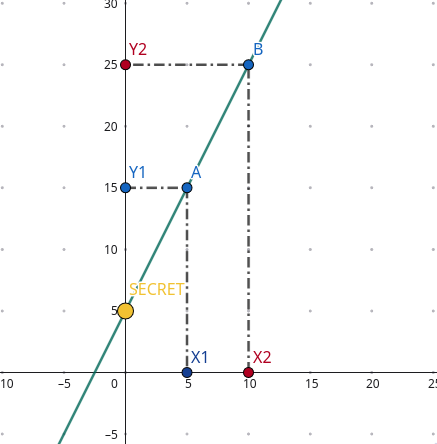
\includegraphics[width=0.4\linewidth]{images/schema_2_n.png}
    \caption{Spiegazione grafica dello schema $(2, n)$}
    \label{fig:schema_2_n}
\end{figure}

Dalla \autoref{fig:schema_2_n}, il segreto coincide con $y(0)$, ossia il punto $(0, S)$.

Lo schema procede così:

\begin{itemize}
    \item Il dealer sceglie u.a.r. un coefficiente $a$ e definisce la retta $y(x) = S + a\,x$.
    \item Assegna a ciascun partecipante un punto sulla retta: il partecipante $i$ riceve $P_i = (x_i, y(x_i))$ (con $x_i$ anche scelto a caso).
    \item Per ricostruire $S$, è sufficiente che due partecipanti forniscano i punti $P_i = (x_i, y_i)$ e $P_j = (x_j, y_j)$; interpolando la retta si ottiene
    \[
    S = y(0) = y_j + \frac{-x_j}{x_i - x_j}(y_i - y_j)
    \]
\end{itemize}

\begin{tcolorbox}[title=Retta passante per due punti, colback=green!5, colframe=green!50!black, fonttitle=\bfseries]
Dati due punti $P_i = (x_i, y_i)$ e $P_j = (x_j, y_j)$, l'unica retta passante per questi punto è data da:
\[
\frac{y - y_j}{y_i - y_j} = \frac{x - x_j}{x_i - x_j} \to y = y_j +  \frac{x - x_j}{x_i - x_j}(y_i - y_j)
\]
\end{tcolorbox}

\begin{example}
    Siano $P_i = (3, 84)$ e $P_j = (1, 54)$, allora
    \[
    S = y_j + \frac{-x_j}{x_i - x_j}(y_i - y_j) = 54\frac{3}{2} - 84\frac{1}{2} = 39
    \]
\end{example}

\subsection{Estensione a $(t, n)$}

L'idea è codificare $S$ come termine noto di un polinomio di grado $t-1$ definito su un campo finito $\mathbb{F}_q$ (tipicamente $\mathbb{Z}_p$ con $p$ primo e $p>n$\footnote{Se $n = 100$, $p = 101$ è un primo valido.}). In questo modo, qualunque insieme di $t$ punti determina univocamente il polinomio (e quindi $S$), mentre con meno di $t$ punti il segreto rimane perfettamente nascosto.

\begin{enumerate}[itemsep=2pt, topsep=2pt]
    \item Scelta dei parametri: si fissa un campo $\mathbb{F}_q$ con $q>n$.
    \item Generazione: il dealer estrae $a_1,\dots,a_{t-1}\gets_{u.a.r.}\mathbb{F}_q$ e definisce
    \[
        f(x)=S+a_1x+a_2x^2+\cdots+a_{t-1}x^{t-1}\in\mathbb{F}_q[x].
    \]
    \item Distribuzione: si scelgono $x_1,\dots,x_n \in \mathbb{F}_q^*$ distinti e si consegna a ogni partecipante $i$ la quota
    \[
        P_i=(x_i,\,y_i=f(x_i)).
    \]
    \item Ricostruzione: Il dealer riceve un'qualsiasi sottoinsieme di $t$ segreti, e ricostruisce $S$ interpolando il polinomio usando l'interpolazione di Lagrange:
    Dato un insieme di $t$ quote $(x_i,y_i)$ su $f$ (grado $t-1$), il segreto vale
    \[
        S=f(0)=\sum_{i=1}^{t} y_i\,\lambda_i
        \qquad\text{dove}\qquad
        \lambda_i=\prod_{\substack{j=1\\ j\neq i}}^{t}\frac{-x_j}{\,x_i-x_j\,}\in\mathbb{F}_q.
    \]
\end{enumerate}

\textbf{Proprietà.}
\begin{description}
    \item [Correttezza:] $t$ punti determinano univocamente $f$, quindi recuperano $S=f(0)$.
    \item [Perfect Secrecy:] con meno di $t$ punti, per ogni $S'\in\mathbb{F}_q$ esiste un polinomio di grado $t\!-\!1$ coerente con le quote osservate e $f(0)=S'$, dunque le quote non rivelano informazione su $S$.
\end{description}

\begin{example}[Schema $(3, 4)$]
    Sia $\mathbb{F}_{q} = \mathbb{Z}_{101}$, consideriamo il polinomio
    \[
    p(x) = 32 + 52x + 3x^2 \mod 101.
    \]
    I punti condivisi sono: $P_1 = (1, 87),\ P_2 = (2, 47),\ P_3 = (3, 13),\ P_4 = (4, 86)$.
    Calcoliamo $S$ usando $P_1, P_2, P_3$.
    \[
        S = p(0) = \sum_{i=1}^3 y_i\lambda_i = 87 \cdot 3 + 47 \cdot(-3) + 13 \cdot 1 \mod 101 = 32.
    \]   
\end{example}

\subsection{Secret Sharing $(2, 2)$ for RSA}

L'obiettivo è suddividere l'esponente segreto $d$ in due quote, così che nessuna parte possa operare da sola; firma e decifratura si ottengono solo cooperando, senza mai ricostruire $d$ per intero.

Sia $N=pq$ con $\phi(N)=(p-1)(q-1)$ e $e\cdot d \equiv 1 \pmod{\phi(N)}$.

\paragraph{Setup (divisione del segreto).}
Si sceglie $d_1 \gets_{u.a.r.} \mathbb{Z}_{\phi(N)}$ e si pone $d_2 \equiv d - d_1 \pmod{\phi(N)}$, in modo che $d_1 + d_2 \equiv d \pmod{\phi(N)}$.

\paragraph{Firma/Decifratura.}
La Parte 1 calcola $\sigma_1 \equiv H(m)^{d_1} \pmod N$, la Parte 2 calcola $\sigma_2 \equiv H(m)^{d_2} \pmod N$, e l’aggregatore ottiene
\[
\sigma \equiv \sigma_1 \cdot \sigma_2
\equiv H(m)^{d_1}\cdot H(m)^{d_2}
\equiv H(m)^{\,d} \pmod N.
\]
La verifica è quella standard RSA: $\sigma^e \equiv H(m) \pmod N$.
In modo analogo per la decifratura: $c^{d_1}\cdot c^{d_2} \equiv c^{d} \pmod N$.

\newpage
\section{Secret Sharing for Secure Multiparty Computation}

\begin{definition}[SMC]
    \text{SMC} sta per \textbf{Secure Multiparty Computation} è consiste nel calcolare il risultato di una funzione che prende in input dati da più persone, \textit{senza che nessuno debba rivelare il proprio dato agli altri}.

    Sia $\mathcal{P} = \{P_1, P_2, \dots, P_n\}$ un insieme di $n$ parti distinte. Ogni parte $P_i$ detiente un valroe di input privato denotato con $z_i$. L'obiettivo del protocollo è calcolare una funzione deterministica $f$ sugli input di tutte le parti:
    \[
    y = f(z_1, z_2, \dots, z_n)
    \]
    soggetta ai seguenti vingoli:
    \begin{description}
        \item[Correttezza e Pubblicazione:] Il risultato $y$ viene calcolato correttamente ed è reso pubblico.
        \item[Privacy degli Input:] Nessuna informazione riguradante i valori privati $z_i$ viene rivelata durante il processo di calcolo, ad eccezione di quanto può essere logicamente dedotto dal risultato finale $y$ stesso.
    \end{description}
    A noi ci interessa nello specifico il caso dell'aggregazione lineare (addizione pesata), ossia
    \[
    f(z_1, z_2, \dots, z_n) = \sum_{i = 1}^{n} \alpha_iz_i = \alpha_1z_1 + \alpha_2z_2 + \dots + \alpha_nz_n
    \]
    dove $\alpha_i$, rappresentano dei coefficienti o pesi.

    Se la funzione $f$ appartiene a questa classe, la SMC può essere implementata in modo molto efficiente utilizzando schemi di \textit{secret sharing}.
\end{definition}

Prima di proseguire, è necessario introdurre la \textbf{proprietà omomorfica}, principio fondamentale alla base della SMC.

\begin{definition}[Proprietà Omomorfica]
    Siano dati due segreti distinti, $S_F$ e $S_G$. Nello schema di Shamir, questi segreti sono nascosti nei temini noti di due polinomi $f(x)$ e $g(x)$ di grado $t - 1$, tali che:
    \[
    f(0) = S_F \quad \text{e} \quad g(0) = S_G
    \]
    Ogni partecipanti $i$ (con $i = 1, \dots, n$) possiede una \textbf{share} (quota) per ciascun segreto, calcolato valutando i polinomi nel punto $i$.
    \[
    y_{i, F} = f(i) \qquad \text{e} \qquad y_{i, G} = g(i)
    \]

    La proprietà omomorfica afferma che \textbf{la somma delle share è uguale alla share della somma}.
    
    \[
    y_{i,\text{somma}} = y_{i, F} + y_{i, G} = f(i) + g(i) = (f + g)(i)
    \]

    Cioè, il valore $y_{i,\text{somma}}$ corrisponde esattamente alla valutazione nel punto $i$ del polinomio somma $(f + g)(i)$. Quindi, poiché l'operazione di somma tra polinomi preserva il termine noto (la somma dei termini noti è il termine noto del polinomio somma), il segreto ricostruibile dalle nuove quote aggregate sarà:
    \[
    S_{\text{totale}} = (f + g)(0) = f(0) + g(0) = S_F + S_G 
    \]

    Questo dimostra che rivelare le quote composite $y_{i,\text{somma}}$ permette di ricostruire la \textbf{somma dei segreti} $(S_F + S_G)$, \textbf{ma non rivela alcuna informazione} sui singoli segreti originali $S_F$ e $S_G$.
\end{definition}

\newpage

\begin{example}
    Consideriamo il seguente esempio, siano:
    \begin{itemize}
        \item \textbf{Modulo:} $p = 11$ (campo finito $\mathbb{Z}_{11}$)
        \item \textbf{Soglia:} $t = 2$ (bastano 2 quote per ricostruire)
        \item \textbf{Segreti scelti:} $S_F = 3$, $S_G = 4$
    \end{itemize}

    Il Dealer genera due polinomi casuali di grado $t-1 = 1$:
    \begin{align*}
        f(x) &= 3 + 2x \pmod{11} \quad (\text{nasconde } S_F) \\
        g(x) &= 4 + 5x \pmod{11} \quad (\text{nasconde } S_G)
    \end{align*}

    Ogni partecipante $P_i$ riceve le quote $f(i)$ e $g(i)$ e calcola localmente la loro somma.

    \begin{table}[h!]
    \centering
    \resizebox{\textwidth}{!}{%
        \renewcommand{\arraystretch}{1.5}
        \begin{tabular}{|c|c|c|c|c|}
            \hline
            \textbf{Utente} ($x$) & \textbf{Quota Segreto F} ($y_{i,F}$) & \textbf{Quota Segreto G} ($y_{i,G}$) & \textbf{Quota Somma} ($y_{i,\text{sum}}$) \\
            \hline
            $P_1$ ($x=1$) & $3 + 2(1) = \mathbf{5}$ & $4 + 5(1) = \mathbf{9}$ & $5 + 9 = 14 \equiv \mathbf{3} \pmod{11}$ \\
            \hline
            $P_2$ ($x=2$) & $3 + 2(2) = \mathbf{7}$ & $4 + 5(2) = 14 \equiv \mathbf{3}$ & $7 + 3 = 10 \equiv \mathbf{10} \pmod{11}$ \\
            \hline
            $P_3$ ($x=3$) & $3 + 2(3) = \mathbf{9}$ & $4 + 5(3) = 19 \equiv \mathbf{8}$ & $9 + 8 = 17 \equiv \mathbf{6} \pmod{11}$ \\
            \hline
        \end{tabular}%
    }
    \caption{Calcolo delle quote aggregate}
    \end{table}

    Le nuove quote calcolate sono i punti: $(1, 3)$, $(2, 10)$, $(3, 6)$.
    Questi punti appartengono al \textbf{polinomio somma} teorico:
    \[
    h(x) = f(x) + g(x) = (3+2x) + (4+5x) = \mathbf{7 + 7x} \pmod{11}
    \]
    Il termine noto di $h(x)$ è \textbf{7}, che corrisponde esattamente alla somma dei segreti originali ($3+4$).

    \textbf{Verifica della consistenza per $P_2$:}
    \[
    y = 7 + 7(2) = 7 + 14 = 21 \equiv \mathbf{10} \pmod{11} \quad \text{(Corretto!)}
    \]
    Inoltre, presi due punti, $(1, 3)$ e $(2, 10)$, la retta passante per questi punti è:
    \[
        y = 10 + \frac{x - 2}{1 - 2}(3 - 10) = 10 + 7x - 14 \mod 11 = 7x - 4 \mod 11 = 7x + 7  
    \]
\end{example}

\subsection{TTP vs SMC}

Tradizionalmente, per eseguire un'aggregazione, tutti gli utenti inviano i dati in chiaro a un server centrale, una \textbf{Trusted Third Party (TTP)}. Per calcolare, ad esempio, una somma, tale ente deve accedere a tutti i dati privati. Se la TTP viene compromessa o si comporta in modo malevolo, la privacy di tutti è a rischio. Questo modello è semplice e funziona, ma non offre garanzie di riservatezza nei confronti di chi esegue il calcolo.

In alternativa, si adotta un insieme di server distribuiti, detti \textit{Privacy Peers}, che operano su dati condivisi tramite secret sharing. L'utente $P_1$, anziché inviare $z_1$ in chiaro, lo suddivide in quote e ne invia una a ciascun peer. Ogni peer riceve soltanto frammenti privi di significato presi singolarmente. Ciascun peer somma localmente le quote ricevute, ottenendo una quota del risultato finale $Share(\mathrm{RES})$, senza mai vedere i dati originali; il risultato si ricostruisce solo combinando un numero sufficiente di quote.

\subsection{Problemi di Implementazione}
Per utilizzare il sistema in sicurezza è opportuno imporre alcuni vincoli operativi.
\begin{description}
    \item[Input peers ($n$): almeno 3.] Con soli 2 partecipanti, A e B, se il risultato aggregato (es. la somma) è pubblico, A può sottrarre il proprio contributo e dedurre esattamente quello di B. Con 3 o più partecipanti questo non è più possibile.
    \item[Privacy peers ($k$): almeno 2.] Un solo privacy peer riceverebbe abbastanza quote da ricostruire i segreti. Aumentare il numero di privacy peers riduce il rischio di collusione.
    \item[Chi sono i privacy peers.] Gli stessi input peers possono fungere da privacy peers: non serve acquistare server esterni; gli utenti possono scambiarsi le quote tra loro ed eseguire il calcolo distribuito.
\end{description}

\subsection{Costruzione}

Basato sullo schema di Shamir, il protocollo permette di calcolare la somma degli input senza rivelarli. Il processo si articola in tre fasi distinte.

\begin{description}
    \item[1. Input Peer $i$ (Fase di invio)] 
    L'utente $i$ possiede un dato privato $z_i$ (es. il proprio salario).
    L'utente genera un polinomio casuale $p_i(x)$ di grado $t-1$, imponendo che il termine noto sia il proprio segreto:
    \[
        p_i(0) = z_i
    \]
    A questo punto, l'utente valuta il polinomio nei punti corrispondenti agli indici dei server e invia le quote in modo privato, non dovendo comunicare tra loro né scambiarsi chiavi.
    \begin{align*}        
        &\text{Invia $p_i(1)$ al Privacy Peer 1} \\
        &\text{Invia $p_i(2)$ al Privacy Peer 2} \\
        &\vdots \\ 
        &\text{Invia $p_i(k)$ al Privacy Peer $k$} \\ 
    \end{align*}
    \item[2. Privacy Peer $m$ (Fase di calcolo)]
    Ogni server di calcolo riceve una quota da ciascun utente, $p_1(m), p_2(m), \dots, p_n(m)$.
    Calcola la somma aritmetica delle quote ricevute. Grazie alla proprietà omomorfica, questa somma corrisponde a un punto del "polinomio somma":
    \[
        \text{RES}(m) = \sum_{j=1}^{n} p_j(m) = p_1(m) + p_2(m) + \dots + p_n(m)
    \]
    Il server pubblica il risultato parziale aggregato $\text{RES}(m)$. Questo valore, da solo, non rivela nulla sui dati originali.
    \item[3. Public (Fase di ricostruzione)]
    Questa fase può essere eseguita da chiunque abbia accesso ai risultati pubblicati. Si raccolgono almeno $t$ valori pubblici $\text{RES}(m)$ dai vari Privacy Peers. Utilizzando l'interpolazione di Lagrange, si ricostruisce il termine noto del polinomio risultante, che corrisponde esattamente alla somma totale degli input:
    \[
        Z_{\text{totale}} = \sum_{i=1}^{n} z_i
    \]

    Se si sceglie di usare tutti i privacy peer per la ricostruzione, allora si può usare l'approccio banale di secret sharing.
\end{description}

\newpage

\begin{example}
    Consideriamo un esempio basato su uno schema di secret sharing $(3,3)$ in cui i privacy peer coincidono con gli input peer. Trattandosi di uno schema $(k,k)$, è sufficiente adottare l'approccio banale.

    Consideriamo 3 parti ($P_1, P_2, P_3$) che vogliono calcolare la somma dei loro valori segreti ($14, 26, 38$) utilizzando l'aritmetica \textbf{modulo 100}.

    \begin{table}[h!]
        \centering
        \setlength{\tabcolsep}{4pt} 
        
        \begin{tabular}{l ccc c} 
            \toprule
            & \multicolumn{3}{c}{\textbf{Quote inviate a...}} & \\
            \cmidrule(lr){2-4}
            \textbf{Mittente ($Z_i$)} & \textbf{Party 1} & \textbf{Party 2} & \textbf{Party 3} & \textbf{Verifica} \\ 
            \midrule
            
            \textbf{Party 1} ($14$) & $\mathbf{34}$ & $89$ & $91$ & \footnotesize ($34+89+91 \equiv 14$) \\
            
            \textbf{Party 2} ($26$) & $66$ & $\mathbf{11}$ & $49$ & \footnotesize ($66+11+49 \equiv 26$) \\
            
            \textbf{Party 3} ($38$) & $47$ & $51$ & $\mathbf{40}$ & \footnotesize ($47+51+40 \equiv 38$) \\
            
            \midrule
            \textbf{SOMMA LOCALE} & $\downarrow$ & $\downarrow$ & $\downarrow$ & \\
            \textbf{(Risultato)} & $\mathbf{47}$ & $\mathbf{51}$ & $\mathbf{80}$ & \\
            \bottomrule
        \end{tabular}
        \caption{Matrice di scambio delle quote (Modulo 100). Sulla diagonale in grassetto le quote trattenute.}
    \end{table}
    
    Si sommano i risultati parziali pubblicati dai tre nodi:
    \[
    \text{Totale} = R_1 + R_2 + R_3 = 47 + 51 + 80 = 178 \equiv \mathbf{78} \pmod{100}
    \]
    Il risultato corrisponde esattamente alla somma degli input segreti ($14 + 26 + 38 = 78$).
\end{example}

\newpage

\section{Verifiabile Secret Sharing}

Nei modelli di \textit{secret sharing} tradizionali, si assume che tutti i partecipanti (sia il Dealer che distribuisce i pezzi del segreto, sia le Parti che li conservano) siano onesti. Tuttavia, questo modello presenta dei limiti critici:
\begin{description}
    \item[Dealer Malvagio:] Non c'è modo di verificare se il Dealer stia distribuendo quote coerenti tra loro.
    \item[Parti Corrotte:] Non si può rilevare se un partecipante riveli una quota falsa al momento della ricostruzione del segreto.
\end{description}

La VSS introduce la possibilità per ogni partecipante di verificare matematicamente la validità delle quote ricevute senza dover conoscere il segreto intero. Questo avviene solitamente attraverso i Commitments.

In questo capitolo verranno discurssi 3 schemi principali:

\begin{description}
    \item[Schema di Feldman (1987):] Il primo schema non interattivo basato sulla difficoltà del logaritmo discreto. È efficiente ma solo computazionalmente sicuro, poiché il commitment del segreto $(g^s)$ potrebbe trapelare informazioni se il segreto è molto piccolo.

    \item[Schema di Pedersen (1991):] Risolve il problema della sicurezza di Feldman utilizzando commitments perfettamente sicuri (\textbf{hiding}), garantendo che nessuna informazione sul segreto venga trapelata, a patto di una sicurezza computazionale nel vincolo (\textbf{binding}).

    \item[Distributed Key Generation (DKG):] Una tecnica avanzata che permette a un gruppo di generare una coppia di chiavi (pubblica/privata) in modo che la chiave pubblica sia nota a tutti, ma nessuno conosca la chiave privata completa finché non è necessario.
\end{description}

\begin{definition}[Commitment]
    Un \textbf{commitment (impegno)} è un protocollo che permette a un utente di \textit{sigillare} un valore segreto, rendendolo pubblico in una forma indecifrabile per poi rivelarlo in un secondo momento.

    Per essere considerato valido, un commitment deve soddisfare due proprità fondamentali:

    \begin{description}
        \item[Hiding (Segretezza):] Il ricevitore non deve essere in grado di estrarre alcuna informazione sul valore originale guardando solo l'impegno pubblico.
        \item[Binding (Vincolo):] Una volta inviato l'impegno, il mittente non può più cambiare idea o modificare il valore originale; può solo rivelare quello che ha inizialmente \textit{sigillato}. 
    \end{description}
\end{definition}


\begin{figure}[ht!]
    \centering
    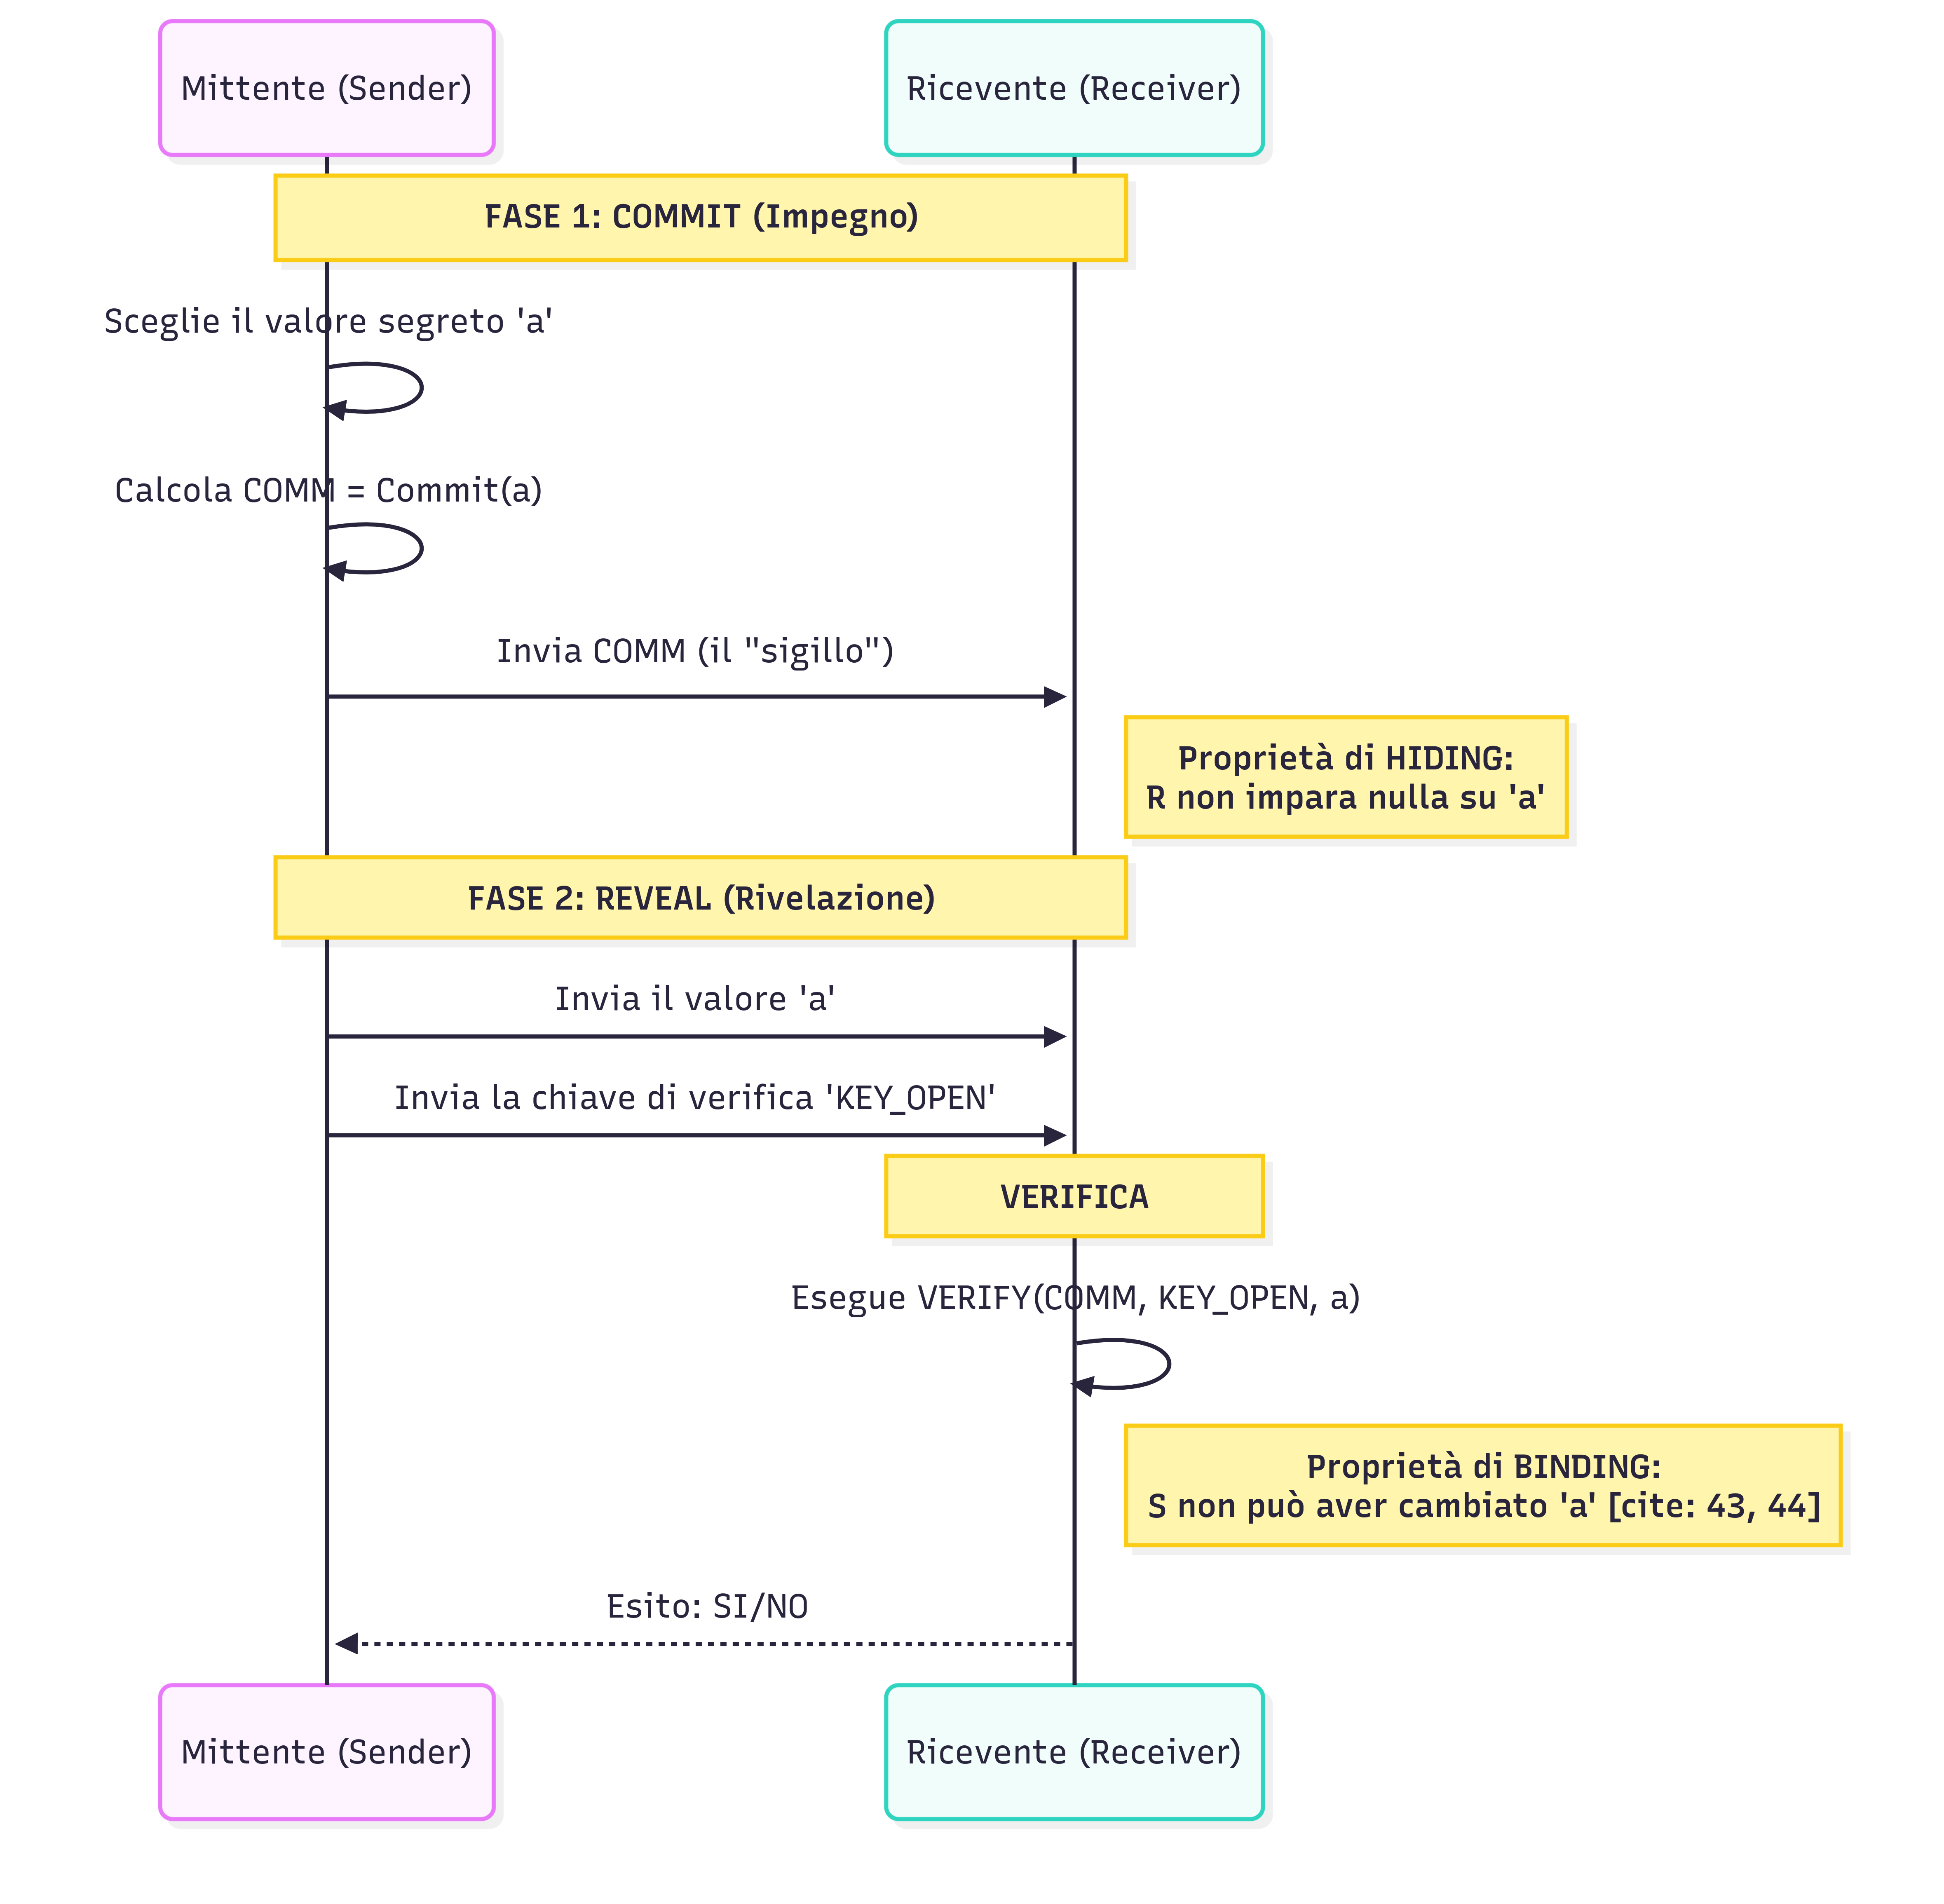
\includegraphics[width=0.48\linewidth]{images/vss_commit_phase.png}
    \caption{Processo di Commitment}
    \label{fig:commitment}
\end{figure}

\subsection{Feldman Scheme}

Lo schema di Feldman, proposto nel 1987, è stato il primo schema di Verifiable Secret Sharing (VSS) di tipo non interattivo. Si basa sull'estensione del classico schema di Shamir, aggiungendo una fase di verifica basata sulla difficoltà del logaritmo discreto.

Si articola di due figure chiave: il \textbf{Dealer} (chi distribuisce) e il \textbf{Verifier} (chi riceve).

\begin{description}
    \item[Dealer:] Come nello schema classico di Shamir, il Dealer crea un polinomio $p(x)$ di grato $t-1$, dove il termine noto è il segreto $S$:
    \[
        p(x) = S + a_1x + a_2x^2 + \dots + a_{t-1}x^{t-1}
    \]
    Invia poi a ogni partecipante $i$ la propria quota privata $y_i = p(x_i)$. Infine, pubblica tutti i commitment calcolati come potenze di un generatore $g$ modulo un numero primo $p$:
    \begin{align*}
        &c_0 = g^S \mod p \\
        &c_1 = g^{a_1} \mod p \\
        &\vdots \\
        &c_{t-1} = g^{a_{t-1}} \mod p \\
    \end{align*}
    \item[Verifier:] Ogni partecipante $i$, ricevuta la sua quota $(x_i, y_i)$, può verificare se il Dealer è stato onesto confrontando la quota con i commit pubblici. Il partecipante controlla se la seguente uguaglianza è verificata:
    \begin{align*}
        c_0 \cdot c_1^{x_i} \cdot c_2^{x_i^2} \cdots c_{t-1}^{x_i^{t-1}} &= (g^S) \cdot (g^{a_1})^{x_i} \cdot (g^{a_2})^{x_i^2} \cdots (g^{a_{t-1}})^{x_i^{t-1}} \\
        &= g^S \cdot g^{a_1 x_i} \cdot g^{a_2 x_i^2} \cdots g^{a_{t-1} x_i^{t-1}} \\
        &= g^{\,S + a_1 x_i + a_2 x_i^2 + \cdots + a_{t-1} x_i^{t-1}} \\
        &= g^{p(x_i)} = g^{y_i}
    \end{align*}
    Se l'uguaglianza è verificata, allora il Dealer è onesto.
    
    Inolte, durante la fase di ricostruzione del segreto, i partecipanti si \textbf{verificano reciprocamente} per individuare eventuali cheater. Quando il partecipante $i$ rivela la propria quota $y_i$ per la ricostruzione, gli altri confrontano il valore con i commitment pubblici ($c_j$) pubblicati dal Dealer all'inizio, verificando che la quota corrisponda a quanto impegnato. Questo consente di individuare e bloccare quote false durante la ricostruzione.
    \end{description}

    Purtroppo lo schema è solo computazionalmente sicuro (a differenza di Shamir, che è incondizionatamente sicuro) poiché si basa sulla difficoltà del logaritmo discreto. Inoltre, il valore pubblico $c_0 = g^{S}$ può trapelare informazione sul segreto: se $S$ proviene da un dominio piccolo (ad es. $S \in [1,1000]$), un avversario può eseguire un attacco a dizionario calcolando $g^1, g^2, \dots$ fino a trovare $c_0$. Il commitment non è quindi \textit{perfectly hiding}.

    Per rendere lo schema più robusto, è consigliato utilizzare numeri primi tali che $p = 2q + 1$ con $p,\ q$ primi, e di operare all'interno di sottogruppi di ordine $q$ per limitare le informazioni che trapelano.

\newpage

\subsection{Pedersen Scheme}

Lo schema di Pedersen (1991) nasce proprio per risolvere il limite principale di Feldman: il fatto che il commitment pubblico $c_0=g^S$ possa rivelare informazioni sul segreto (specialmente se il segreto è piccolo).

Mentre Feldman è solo \textbf{computazionalmente} sicuro, Pedersen introduce un sistema \textbf{perfectly hiding}.

Il commitment di Feldman funziona in quanto omomorfico, infatti: 
\[
    Commit(a+b) = Commit(a) \cdot Commit(b) \implies g^{a + b} = g^a \cdot g^b \mod p
\]

Nello schema di Pederson, invece di usare un solo generatore $g$, ne vengono usati due, $g$ e $h$, tali che nessuno conosca il logaritmo discreto di $h$ rispetto a $g$ $(\log_g(h))$.

\begin{definition}[Pederson's Commitment]
    Per impegnarsi a un valore $a$, il mittente sceglie un numero casuale $r$ e calcola:
    \[
    Commit(a; r) = g^ah^r \mod p
    \]
    Questo commitment è omomorfico, infatti:
    \begin{proof}
        \[
            Commit(a + b;\ r_a + r_b) = g^{a+b}h^{r_a + r_b} = g^ah^{r_a} \cdot g^bh^{r_b} = Commit(a; r_a) \cdot Commit(b; r_b)
        \]
    \end{proof}

    \textbf{Proprietà:}
    \begin{description}
        \item[Perfecty Hiding] Anche se hai una potenza di calcolo infinita, non puoi scoprire $a$ perché, per ogni possibile valore $a'$, esiste un valore $r'$ che rende il commitment valido.
        Formalmente, $\forall a' \neq a\ \nexists!\ r'$ tale che
        \[
            Commit(a'; r') = g^{a'}h^{r'} = g^ah^r = Commit(a; r)
        \]
        \item[Computationally Binding:] Il mittente non può cambiare $a$ dopo aver inviato il commitment, a meno di non saper risolvere il problema del logaritmo discreto (ovvero conoscere $w$ tale che $h=g^w$)
        \begin{proof}
            Supponiamo per assurdo che si conosca $w = \log_g(h) \implies h = g^w$. 
            Un utente ha creato un commitment per un valore $a$ usando un valore casuale $r$,
            \[
                Commit(a;r) = g^ah^r
            \]
            Vuole ora trovare un nuovo valore $r'$ che gli permetta di sostenere di essersi impegnato su un valore $a' \neq a$, ossia che valga l'uguaglianza
            \begin{align*}
                g^ah^r = g^{a'}h^{r'} 
                &\implies g^ag^{wr} = g^{a'}g^{wr'} \\ 
                &\implies g^{a + wr} = g^{a' + wr'} \\
                &\implies a + wr = a' + wr' \mod q \\
                &\implies r' = w^{-1}a - a' + wr \mod q
            \end{align*}
            Quindi, conoscendo $w$ è possibile calcolare $r'$ per \textbf{qualsiasi} $a'$. Questo significa che il commitment non vincola a nulla (nessun binding).
        \end{proof}
    \end{description}
\end{definition}

\newpage
\begin{tcolorbox}[title=Nota, colback=red!5, colframe=red!50!black, fonttitle=\bfseries]
Non è possibile garantire in contemporanea sia la \textit{perfectly hiding} che la \textit{perfectly binding}.
\end{tcolorbox}

Come lo schema di Feldman, anche lo schema di Pedersen si articola di due figure chiave: il \textbf{Dealer} e il \textbf{Verifier}.

\begin{description}
    \item[Dealer:] Il Dealer genera due polinomi randomici $f(x)$ e $g(x)$ di grado $t-1$, dove il termine noto $f(0) = S$ e il termine noto $g(0) = r$. 
    \begin{align*}
        f(x) &= S + a_1x + a_2x^2 + \dots + a_{t-1}x^{t-1}\\        
        g(x) &= r + b_1x + b_2x^2 + \dots + b_{t-1}x^{t-1}   
    \end{align*}
    Invia poi a ogni partecipante $i$ una \textit{doppia quota} $(x_i, y_i = f(x_i))$ e $(x_i, z_i = g(x_i))$. Infine, pubblica tutti i commitment calcolati come prima, ossia
    \begin{align*}
        &c_0 = g^Sh^r \mod p \\
        &c_1 = g^{a_1}h^{b_1} \mod p \\
        &\vdots \\
        &c_{t-1} = g^{a_{t-1}}h^{b_{t-1}} \mod p \\
    \end{align*}
    \item[Verifier:] Ogni partecipante $i$, ricevuta la sua \textit{doppia quota} $(x_i, y_i, z_i)$, può verificare se il Dealer è stato onesto confrontando la quota con i commit pubblici. Il partecipante controlla se la seguente uguaglianza è verifica:
    \begin{align*}
        c_0 \cdot c_1^{x_i} \cdot c_2^{x_i^2} \cdots c_{t-1}^{x_i^{t-1}} &= (g^Sh^r) \cdot (g^{a_1}h^{b_1})^{x_i} \cdot (g^{a_2}h^{b_2})^{x_i^2} \cdots (g^{a_{t-1}}h^{b_{t-1}})^{x_i^{t-1}} \\
        &= g^S \cdot g^{a_1 x_i} \cdot g^{a_2 x_i^2} \cdots g^{a_{t-1} x_i^{t-1}} \cdot h^r \cdot h^{b_1 x_i} \cdot h^{b_2 x_i^2} \cdots h^{b_{t-1} x_i^{t-1}} \\
        &= g^{\,S + a_1 x_i + a_2 x_i^2 + \cdots + a_{t-1} x_i^{t-1}} \cdot h^{\,r + b_1 x_i + b_2 x_i^2 + \cdots + b_{t-1} x_i^{t-1}}\\
        &= g^{f(x_i)}h^{g(x_i)} = g^{y_i}h^{z_i}
    \end{align*}
\end{description}

\begin{table}[h]
\centering
\renewcommand{\arraystretch}{1.5}
\resizebox{\textwidth}{!}{%
    \begin{tabular}{|l|p{6cm}|p{6cm}|}
    \hline
    \textbf{Caratteristica} & \textbf{Feldman VSS} & \textbf{Pedersen VSS} \\ \hline
    \textbf{Hiding (Privacy)} & \textbf{Computazionale}: il valore $g^s$ può rivelare informazioni se il segreto $s$ è piccolo. & \textbf{Perfetto}: l'impegno $g^a h^r$ può corrispondere matematicamente a qualunque valore. \\ \hline
    \textbf{Binding (Vincolo)} & \textbf{Perfetto}: matematicamente esiste un solo esponente possibile per un dato impegno pubblico. & \textbf{Computazionale}: il vincolo dipende dalla difficoltà di risolvere il logaritmo discreto $log_g h$. \\ \hline
    \textbf{Natura del segreto} & Basato sulla generazione di un singolo polinomio casuale $p(x)$ di grado $t-1$. & Basato sulla generazione di due polinomi casuali $f(x)$ e $f'(x)$. \\ \hline
    \end{tabular}%
}
\caption{Confronto tra gli schemi di Verifiable Secret Sharing di Feldman e Pedersen.}
\end{table}

\newpage
\subsection{Distributed Key Generation}

Per garantire che lo schema di Pedersen sia effettivamente sicuro, dobbiamo risolvere l'ultimo grande ostacolo: la generazione del valore $h$. Se il Dealer generasse $h=g^w$ conoscendo $w$, potrebbe barare calcolando commitments che collidono e violando la proprietà di binding. Dobbiamo quindi trovare un modo per generare $h$ senza che nessuno ne conosca la chiave privata $w$.

La soluzione a questo problema è la \textbf{Distributed Key Generation - DKG}, una tecnica che permette a un insieme di nodi di collaborare per creare una coppia di chiavi $(Pub_K, Priv_k)$, dove tutti conoscono la chiave pubblica $(h = g^w)$ e nessuno conosce quella privata $(w)$.

Oltre alla VSS, la DKG è essenziale in molti sistemi crittografici moderni:
\begin{enumerate}
    \item Sistemi basati su Logaritmo Discreto: Come El Gamal o la Crittografia Basata sull'Identità (IBE).
    \item Rivelazione posticipata: Quando una chiave privata deve essere rivelata solo al verificarsi di condizioni speciali.
    \item Funzioni distribuite: Quando la chiave privata non viene mai rivelata, ma è necessario calcolare funzioni che dipendono da essa.
\end{enumerate}

Il metodo più comune è il \textbf{Pedersen DKG (1991)}, che è essenzialmente un'applicazione ricorsiva dei concetti di Secret Sharing visti finora.

In questo schema, non esiste un'autorità centrale o un Trusted Third Party (TTP): ogni partecipante agisce contemporaneamente come "Dealer" di una propria parte del segreto e come "Parte" che riceve quote dagli altri.

Vediamo nel dettaglio come funziona per uno schema $(t, n)$.

\begin{description}
    \item[FASE 1: Generazione Locale e Polinomi] Ogni partecipante $i$,genera un polinomio casuale $p_i(x)$ di grado $t-1$, dove il termine noto è il segreto $S_i = a_{0,i}$
    \[
        p_i(x) = S_i + a_{1,i}x + a_{2,i}x^2 + \dots + a_{t-1,i}x^{t-1}\\ 
    \]
    \item[FASE 2: Scambio delle Quote] Ogni partecipante distribuisce le quote del proprio segreto agli altri. Quindi il partecipante $i$ riceve $n-1$ quote e distribuisce a sua volta $n-1$ quote del proprio segreto.
    \item[FASE3: Calcolo Quota Finale e Commitiments] Ora ogni partecipante somma ciò che ha ricevuto per ottenere la sua quota del segreto globale:
    \[
    y_i = \sum_{j = 1}^{n}p_j(i)
    \]
    Infine, ogni parte pubblica l'impegno del proprio segreto locale $c_i = g^{a_{0,i}}$.
\end{description}

In conclusione, il segreto globale $S=\sum_{i=1}^{n} a_{0,i}$ non è noto a nessuno, poiché ogni $a_{0,i}$ resta privato. La chiave pubblica associata è $g^{S}$, calcolabile da tutti come
\[
g^{S}=\prod_{i=1}^{n} g^{a_{0,i}}=\prod_{i=1}^{n} c_i.
\]
Infine, ogni partecipante può verificare la correttezza della propria quota rispetto ai commitment pubblici divulgati durante la DKG.

\newpage

Quindi per poter utilizzare lo schema di \textbf{Pedersen VSS} in modo sicuro, è necessario che il parametro pubblico $h$ sia generato tramite il protocollo \textbf{Pedersen DKG}.

\begin{description}
    \item[Fase 0 (DKG):] I partecipanti collaborano per generare $h=g^w$ senza che $w$ venga rivelato a nessuno.
    \item[Fase 1 (Commitment):] Si usa questo $h$ per creare impegni sicuri del tipo $g^ah^r$.
    \item[Fase 2 (VSS):] Il Dealer distribuisce le quote del segreto usando i due polinomi $f(x)$ e $g(x)$, permettendo a tutti di verificare l'onestà tramite gli impegni basati su $g$ e $h$.
\end{description}

\begin{example}
    In questo scenario, 4 partecipanti ($n=4$) collaborano per generare una chiave pubblica comune con una soglia di ricostruzione di 3 persone ($t=3$).

    \textbf{1. Generazione dei Segreti Locali e dei Polinomi} \\
    Ogni partecipante $P_i$ sceglie un proprio segreto casuale $a_{0,i}$ e definisce un polinomio di grado 2 ($t-1$):
    \begin{itemize}
        \item $P_1$ sceglie $a_{0,1}$ e crea $p_1(x) = a_{0,1} + a_{1,1}x + a_{2,1}x^2$
        \item $P_2$ sceglie $a_{0,2}$ e crea $p_2(x) = a_{0,2} + a_{1,2}x + a_{2,2}x^2$
        \item $P_3$ sceglie $a_{0,3}$ e crea $p_3(x) = a_{0,3} + a_{1,3}x + a_{2,3}x^2$
        \item $P_4$ sceglie $a_{0,4}$ e crea $p_4(x) = a_{0,4} + a_{1,4}x + a_{2,4}x^2$
    \end{itemize}

    \textbf{2. Scambio Sicuro delle Quote} \\
    Ogni partecipante calcola i valori del proprio polinomio nei punti $1, 2, 3, 4$ e li invia agli altri. Ad esempio, $P_1$ tiene per sé $p_1(1)$ e invia:
    \begin{itemize}
        \item $p_1(2) \to P_2$, \quad $p_1(3) \to P_3$, \quad $p_1(4) \to P_4$
    \end{itemize}
    Contemporaneamente, $P_1$ riceve le quote dagli altri partecipanti: $p_2(1)$, $p_3(1)$ e $p_4(1)$.

    \textbf{3. Calcolo della Quota Finale (Full Share)} \\
    Ogni partecipante somma tutte le quote ricevute (inclusa la propria) per ottenere la sua quota del segreto collettivo $s$:
    \begin{itemize}
        \item $P_1$ calcola $y_1 = p_1(1) + p_2(1) + p_3(1) + p_4(1)$
        \item $P_2$ calcola $y_2 = p_1(2) + p_2(2) + p_3(2) + p_4(2)$
        \item $P_3$ calcola $y_3 = p_1(3) + p_2(3) + p_3(3) + p_4(3)$
        \item $P_4$ calcola $y_4 = p_1(4) + p_2(4) + p_3(4) + p_4(4)$
    \end{itemize}

    \textbf{4. Pubblicazione degli Impegni (Commitments)} \\
    Per permettere la verifica e il calcolo della chiave pubblica, ogni partecipante pubblica l'impegno del proprio segreto:
    \begin{itemize}
        \item Broadcast di: $g^{a_{0,1}}, g^{a_{0,2}}, g^{a_{0,3}}, g^{a_{0,4}}$
    \end{itemize}

    \textbf{5. Conclusione: Il Segreto Condiviso} \\
    Senza che nessuno conosca il segreto totale $s$, il gruppo ha generato:
    \begin{itemize}
        \item \textbf{Segreto Globale (Privato):} $s = a_{0,1} + a_{0,2} + a_{0,3} + a_{0,4}$
        \item \textbf{Chiave Pubblica:} $g^s = g^{a_{0,1}} \cdot g^{a_{0,2}} \cdot g^{a_{0,3}} \cdot g^{a_{0,4}}$
        \item \textbf{Quote di Verifica:} Ogni $y_i$ è una quota valida del segreto $s$
    \end{itemize}
\end{example}

\newpage

\section{Threshold and Policy-Based Cryptography}

In questo capitolo estendiamo il concetto di \textbf{secret sharing}: l'obiettivo non è solo custodire un segreto, ma distribuire l'autorità di eseguire operazioni crittografiche (decifratura e firma) tra più entità, aumentando la resilienza e riducendo i punti di fallimento.
\begin{description}
    \item[Threshold Encryption:] Adattiamo \textbf{ElGamal} in forma threshold, in modo che la decifratura sia possibile solo con la cooperazione di almeno $t$ partecipanti.
    \item[Threshold Signatures:] Permettiamo a un gruppo di generare collettivamente una firma standard e verificabile, ricostruibile solo da insiemi di almeno $t$ partecipanti.
    \item[Policy-Based Schemes:] Generalizziamo le soglie a strutture di accesso (politiche) più ricche, dove insiemi autorizzati di partecipanti possono decifrare/firmare secondo regole prefissate.
\end{description}

\subsection{Threshold Encryption: ElGamal}

L'algoritmo di cifratura di ElGamal trasforma lo scambio di chiavi di Diffie-Hellman in un vero sistema di cifratura. Vediamo il caso del logaritmo discreto (più avanti lo vederemo con le curve ellittiche).

\subsubsection*{ElGamal Classico}

Il sistema di cifratura classico di ElGamal funziona in questo modo: innanzitutto si scelgono un numero $p$ primo molto grande e un generatore $g$ del gruppo ciclico.

\begin{description}
    \item[Generazione delle chiavi:] Si genera la coppia $(SK, PK)$.
    \begin{align*}
        SK &\gets_{u.a.r.}\ \mathbb{Z}_p^* \\
        PK &= g^{SK} \pmod{p}
    \end{align*}
    \item[Cifratura:] Dato $m \in \mathbb{Z}_p^*$, si sceglie $k \gets_{u.a.r.}\ \mathbb{Z}_p^*$ (\textit{chiave effimera}) e si calcolano:
    \begin{align*}
        A &= g^k \pmod{p} \\
        B &= m \cdot PK^k \pmod{p}
    \end{align*}
    Il cifrato è la coppia $(A, B)$.
    \item[Decifratura:] Ricevuto $(A, B)$, si ricava $m$ usando $SK$:
    \begin{align*}
        m &= B \cdot (A^{SK})^{-1} \pmod{p} \\
          &= \frac{B}{A^{SK}} = \frac{m \cdot g^{k\,SK}}{g^{k\,SK}} \pmod{p}
    \end{align*}
\end{description}

\subsubsection*{Threshold ElGamal}

Il sistema classico di cifratura di ElGamal si può estendere in un sistema \textbf{Threshold (a soglia)}. L'idea è che vogliamo cifrare un messaggio in modo che nessuno possa leggerlo da solo, ma sia necessaria la collaborazione di almeno $t$ partecipanti su un totale di $n$.

\begin{description}
    \item[Setup:] Si condivide la chiave privata $SK$ tramite \textbf{Shamir Secret Sharing}. Si fissa un campo $\mathbb{F}_q$ con $q>n$ e si scelgono indici pubblici distinti $x_1,\dots,x_n\in\mathbb{F}_q^*$. Si genera un polinomio $f(x)$ di grado $t-1$ con termine noto $f(0)=SK$, e si consegna a ciascun partecipante $i$ la quota $SK_i=f(x_i)$. Per evitare una TTP e impedire che qualcuno conosca $SK$ per intero, si usa \textbf{Pedersen DKG/VSS}.
        
        Si lavora in $\mathbb{Z}_p^*$ con generatore $g$ di un sottogruppo di ordine $q$ e si pubblica $PK=g^{SK}\pmod{p}$.
    \item[Cifratura:] Il mittente cifra normalmente con $PK$. Sceglie $k\gets_{u.a.r.}\mathbb{Z}_q$ e calcola
    \[
        (A,B)=(g^k \pmod{p},\; m\cdot PK^k \pmod{p}).
    \]
    \item[Decifratura collaborativa:] Almeno $t$ partecipanti cooperano senza ricostruire $SK$. Ogni $i$ calcola la propria \textbf{decifratura parziale} $S_i=A^{SK_i}\pmod{p} = A^{y_i\lambda_i}$ e la invia al combinatore.
    \item[Ricostruzione del messaggio:] Il combinatore esegue l'interpolazione di Lagrange \textbf{all'esponente} (con pesi in $\mathbb{F}_q$):
        \[
            A^{SK}=\prod_{i=1}^{t} S_i\pmod{p},
            \qquad
            \lambda_i=\prod_{\substack{j=1\\ j\neq i}}^{t}\frac{-x_j}{\,x_i-x_j\,}\in\mathbb{F}_q.
        \]
        Ottenuto $A^{SK}$, decifra
        \[
            m=B\cdot \bigl(A^{SK}\bigr)^{-1}\pmod{p}.
        \]
\end{description}

\subsection{Threshold Signatures: RSA}

Il \textbf{Threshold RSA} permette a un gruppo di $n$ entità di produrre congiuntamente una firma, richiedendo la cooperazione di almeno $t$ partecipanti. A differenza di ElGamal, l'adattamento a soglia di RSA è più complesso: l'interpolazione di Lagrange richiede inversioni in $\mathbb{Z}_{\phi(N)}$, ma $\phi(N)$ non deve essere conosciuta (rivelerebbe i fattori di $N$) e, inoltre, $\mathbb{Z}_{\phi(N)}$ non è in generale un campo.

\subsubsection{RSA Classico}

Si scelgono due primi grandi $p,q$, si calcola $N=pq$ e $\phi(N)=(p-1)(q-1)$. Si sceglie $e$ coprimo con $\phi(N)$ e si computa $d=e^{-1}\bmod\phi(N)$.

\begin{description}
    \item[Firma:] Dato un messaggio $m$, si calcola $\sigma=h(m)^d \bmod N$.
    \item[Verifica:] Si accetta se $\sigma^e \equiv h(m) \pmod N$.
\end{description}

\subsubsection{Threshold RSA}

Il nodo critico in Threshold RSA è la combinazione corretta delle firme parziali. Idealmente, il partecipante $i$ dovrebbe contribuire con
\[
    h(m)^{\,d_i\,\lambda_i} \pmod N,
\]
dove i pesi di Lagrange sono
\[
    \lambda_i=\prod_{\substack{j=1\\ j\neq i}}^{t}\frac{-x_j}{\,x_i-x_j\,}
    \qquad\text{e}\qquad
    \lambda_i=\frac{\alpha_i}{\beta_i}\ \text{con}\ \gcd(\alpha_i,\beta_i)=1.
\]
Per ottenere l'esponente frazionario si richiederebbe $\beta_i^{-1}\bmod\phi(N)$:
\[
    h(m)^{\,d_i\,\lambda_i}=h(m)^{\,d_i\,\alpha_i\,\beta_i^{-1}}\pmod N,
\]
ma calcolare $\beta_i^{-1}\bmod\phi(N)$ non è possibile senza conoscere $\phi(N)$ (che rivelerebbe i fattori di $N$). 

Osservazione: se si scelgono indici $x_1,\dots,x_n\in\{1,\dots,n\}$, i denominatori dei $\lambda_i$ dividono $n!$. Si può quindi definire un denominatore comune $\Delta=n!$ per \textit{ripulire} le frazioni.

\begin{description}
    \item[Generazione distribuita:] Si genera congiuntamente $N=pq$ senza rivelare $p,q$ e si condivide l’esponente segreto $d$ tramite Shamir/VSS: ogni partecipante $i$ riceve una quota $y_i=f(x_i)$ di $d$. Si fissano indici pubblici $x_1,\dots,x_n\in\{1,\dots,n\}$ e si pone un denominatore comune $\Delta=n!$. I pesi di Lagrange in $0$ sono
    \[
        \lambda_i=\prod_{\substack{j=1\\ j\neq i}}^{t}\frac{-x_j}{\,x_i-x_j\,}=\frac{\alpha_i}{\beta_i},\qquad \beta_i\mid \Delta,
    \]
    e definiamo $\Lambda_i=\Delta\,\lambda_i\in\mathbb{Z}$.
    \item[Firme parziali:] Ogni partecipante $i$ pubblica
    \[
        \tau_i = h(m)^{\,y_i\,\Lambda_i}\ \bmod N,
    \]
    equivalente a calcolare $h(m)^{y_i}$ e poi elevarlo alla potenza intera $\Lambda_i$.
    \item[Aggregazione:] Il combinatore calcola il prodotto
    \[
        T=\prod_{i=1}^{t}\tau_i \equiv h(m)^{\,\Delta\sum_{i=1}^{t}y_i\lambda_i}\equiv h(m)^{\,\Delta\,d}\pmod N.
    \]
    \item[Rimozione del fattore $\Delta$ (Bézout):] Poiché tipicamente $\gcd(e,\Delta)=1$, si trovano $a,b\in\mathbb{Z}$ tali che $ae+b\Delta=1$ (Algoritmo Euclideo Esteso). La firma è
    \begin{align*}        
        \sigma=h(m)^a\cdot T^{\,b}\ \bmod N 
        &= h(m)^a\cdot h(m)^{b \Delta d} \bmod N \\ 
        &= (h(m)^{ed})^a \cdot h(m)^{b\Delta d} \bmod N \\ 
        &= h(m)^{d(ea + b\Delta)} \bmod N \\ 
        &= h(m)^d \bmod N
    \end{align*}
    \item[Verifica:] Come in RSA classico: $\sigma^e \equiv h(m) \pmod N$.
\end{description}

\subsubsection{Common Modulus Attack}

In threshold RSA, per eliminare il fattore $\Delta$ si usa l'Algoritmo Euclideo Esteso, che richiede $\gcd(e,\Delta)=1$. Questo è un esempio di \textbf{Common Modulus Attack}: se due utenti usano lo stesso modulo $N$ ma esponenti pubblici $e_1,e_2$ coprimi, è possibile calcolare una firma valida per entrambi i sistemi (oppure decifrare il messaggio $m$ senza conoscere la chiave privata).

Siano $e_1,e_2$ tali che $\gcd(e_1,e_2)=1$. Sia $m$ un messaggio e $CT_1 = m^{e_1}\bmod N,CT_2 = m^{e_2}\bmod N$ i respettivi cifrati. Poiché $\gcd(e_1,e_2)=1$, esistono $a,b\in\mathbb{Z}$ tali che $ae_1 + be_2 = 1$. Allora
\[
    CT_1^a \cdot CT_2^b = m^{ae_1 + be_2} \equiv m \pmod N,
\] 
Quindi, senza conoscere $d$, è possibile calcolare $m \equiv m \pmod N$, violando la sicurezza di entrambi i sistemi.

\newpage

\section{Linear Secret Sharing \& Access Control Matrix}

In questa sezione reinterpretiamo lo schema di Shamir in forma lineare e arriviamo alla sua generalizzazione: il Linear Secret Sharing (LSSS). L'obiettivo è condividere un segreto $S$ tra più partecipanti in modo che solo i sottoinsiemi autorizzati (la struttura di accesso) possano ricostruirlo.

Shamir $(t,n)$ su $\mathbb{F}_q$ assegna a ogni partecipante $i$ la quota
\[
    y_i=f(x_i)=S + a_1 x_i + a_2 x_i^2 + \dots + a_{t-1} x_i^{t-1},
\]
che può essere vista come prodotto scalare
\[
    y_i=\underbrace{(\,1,\ x_i,\ x_i^2,\ \dots,\ x_i^{t-1}\,)}_{\text{riga }i}
    \cdot
    \underbrace{(\,S,\ a_1,\ a_2,\ \dots,\ a_{t-1}\,)^T}_{\text{vettore dei coefficienti}}.
\]
Ponendo $r_j=a_j$ si ha
\[
\begin{pmatrix}
1 & x_1 & x_1^2 & \dots & x_1^{t-1} \\
1 & x_2 & x_2^2 & \dots & x_2^{t-1} \\
\vdots & \vdots & \vdots & \ddots & \vdots \\   
1 & x_n & x_n^2 & \dots & x_n^{t-1} \\
\end{pmatrix}
\cdot
\begin{pmatrix}
S \\
r_1 \\
\vdots \\   
r_{t-1} \\
\end{pmatrix}
=
\begin{pmatrix}
y_1 \\
y_2 \\
\vdots \\   
y_n \\
\end{pmatrix},
\]
cioè un sistema lineare $A\mathbf{x}=\mathbf{y}$ con $A$ di tipo Vandermonde, $\mathbf{x}=(S,r_1,\dots,r_{t-1})$ e $\mathbf{y}=(y_1,\dots,y_n)$.

Se un gruppo di $t$ partecipanti si riunisce, può formare un sistema lineare quadrato utilizzando solo le proprie righe e le proprie quote. Se chiamiamo $A'$ la sottomatrice $t \times t$ dei partecipanti presenti, il segreto si trova risolvendo:

\[
    \mathbf{x} = (A')^{-1}\mathbf{y}_{presenti}
\]

Il segreto $S$ è semplicemente la prima entrata del vettore risultato.

\subsection{LSSS e MSP}

Per semplicità, consideriamo uno schema $(3,4)$:
\[
\begin{pmatrix}
1 & x_1 & x_1^2 \\
1 & x_2 & x_2^2 \\
1 & x_3 & x_3^2 \\
1 & x_4 & x_4^2 \\
\end{pmatrix}
\cdot
\begin{pmatrix}
S \\
r_1 \\
r_2 \\
\end{pmatrix}
=
\begin{pmatrix}
y_1 \\
y_2 \\
y_3 \\
y_4 \\
\end{pmatrix}.
\]

Per ricostruire $S$ usando le sole quote di $P_1,P_2,P_4$ si risolve
\[
\begin{pmatrix}
S \\
r_1 \\
r_2 \\
\end{pmatrix}
=
\begin{pmatrix}
1 & x_1 & x_1^2 \\
1 & x_2 & x_2^2 \\
1 & x_4 & x_4^2 \\
\end{pmatrix}^{-1}
\cdot
\begin{pmatrix}
y_1 \\
y_2 \\
y_4 \\
\end{pmatrix}.
\]

Interpretiamo ora le righe dei partecipanti come vettori:
\[
\mathbf{v_1}=(1,x_1,x_1^2),\quad
\mathbf{v_2}=(1,x_2,x_2^2),\quad
\mathbf{v_4}=(1,x_4,x_4^2).
\]
Questi tre vettori generano uno spazio di dimensione $3$.
Poiché il segreto $S$ è associato alla prima colonna, per eliminare la casualità $r_1,r_2$ cerchiamo coefficienti $c_1,c_2,c_3$ tali che
\[
c_1\mathbf{v_1}+c_2\mathbf{v_2}+c_3\mathbf{v_4}=(1,0,0).
\]
Allora
\[
S=(1,0,0)\cdot(S,r_1,r_2)^T=c_1y_1+c_2y_2+c_3y_4,
\]
dove i coefficienti $c_i$ si ottengono risolvendo
\[
\begin{pmatrix}
1 & x_1 & x_1^2 \\
1 & x_2 & x_2^2 \\
1 & x_4 & x_4^2 \\
\end{pmatrix}
\cdot
\begin{pmatrix}
c_1 \\ c_2 \\ c_3
\end{pmatrix}
=
\begin{pmatrix}
1 \\ 0 \\ 0
\end{pmatrix}.
\]

In sintesi, mentre Shamir usa matrici di Vandermonde, la vista lineare consente di usare una qualunque matrice per codificare chi può ricostruire il segreto.

\begin{definition}[LSSS]
    Un \textbf{Linear Secret Sharing Scheme} con soglia $t$ su un campo $\mathbb{F}_q$ condivide un segreto $S$ usando sole trasformazioni lineari.

    Si fissa una matrice $A \in \mathbb{F}_q^{n \times t}$ arbitraria e si costruisce il vettore
    \[
        \mathbf{x} = (S, r_1, \dots, r_{t-1})^T \in \mathbb{F}_q^{t}.
    \]
    Le quote distribuite sono il prodotto
    \[
        \mathbf{y} = A\mathbf{x} =
        \begin{pmatrix}
        y_1 \\
        y_2 \\
        \vdots \\   
        y_n \\
        \end{pmatrix},
        \qquad
        y_i = \mathbf{a}_i \cdot \mathbf{x}
        = a_{i,1} S + \sum_{j=2}^{t} a_{i,j}\, r_{j-1},
    \]
    dove $\mathbf{a}_i = (a_{i,1}, \dots, a_{i,t})$ è la $i$-esima riga di $A$.

    Per un insieme autorizzato $U$ esistono coefficienti $c_i \in \mathbb{F}_q$ tali che
    \[
        \sum_{i \in U} c_i\, \mathbf{a}_i = (1, 0, \dots, 0)
        \quad\Rightarrow\quad
        S = \sum_{i \in U} c_i\, y_i.
    \]

    Questo concetto è conosciuto anche come \textbf{MSP - Monotone Span Program}. Ossia l'insieme $U$ è considerato autorizzato se e solo se le righe della matrice $A$ in loro possesso riescono a generare (fare lo \textbf{span}) il \textbf{vettore target} $(1, 0, 0, \dots)$ attraverso una combinazione lineare. 
    
    Il programma è definito "monotono" perché se un insieme di partecipanti può ricostruire il segreto, anche qualsiasi insieme più grande che li includa può farlo. Non è possibile invece includere negazioni (es. \textit{A e B, ma non C}).

\end{definition}

\begin{example}
    Il \textbf{Trivial Secret Sharing} è un LSSS. Consideriamo uno schema $(3,3)$: le quote si ottengono come
    \[
    \begin{pmatrix}
    1 & -1 & -1 \\
    0 & 1 & 0 \\
    0 & 0 & 1 \\
    \end{pmatrix}
    \cdot
    \begin{pmatrix}
    S \\ r_1 \\ r_2
    \end{pmatrix}
    =
    \begin{pmatrix}
    S - r_1 - r_2 \\ r_1 \\ r_2
    \end{pmatrix},
    \]
    cioè $y_1=S-r_1-r_2$, $y_2=r_1$, $y_3=r_2$.

    Per la ricostruzione, lo span program cerca $c_1,c_2,c_3$ tali che
    \[
    c_1(1,-1,-1)+c_2(0,1,0)+c_3(0,0,1)=(1,0,0).
    \]
    Una scelta valida è $c_1=c_2=c_3=1$, da cui
    \[
    S=c_1y_1+c_2y_2+c_3y_3=(S-r_1-r_2)+r_1+r_2=S.
    \]
\end{example}

\textbf{LSSS è omomorfico}
Siano $S_a$ e $S_b$ due segreti condivisi con la stessa matrice di distribuzione $A$. Definiamo
\[
\mathbf{x_a}=(S_a, r_{1a}, \dots, r_{t-1,a})^T,\qquad
\mathbf{x_b}=(S_b, r_{1b}, \dots, r_{t-1,b})^T,
\]
e le rispettive quote $\mathbf{y_a}=A\mathbf{x_a}$, $\mathbf{y_b}=A\mathbf{x_b}$. Per linearità,
\[
\mathbf{y_a}+\mathbf{y_b}=A\mathbf{x_a}+A\mathbf{x_b}=A(\mathbf{x_a}+\mathbf{x_b})
= A\,(S_a+S_b,\ r_{1a}+r_{1b},\dots, r_{t-1,a}+r_{t-1,b})^T.
\]
Ne segue che, per ogni partecipante $i$, $y_{i,a}+y_{i,b}$ è una quota valida del segreto $S_a+S_b$ rispetto ad $A$.

\newpage

\begin{example}[MSP]
Riscriviamo un MSP su $GF(2)$ (Galois Field, dove l'addizione = XOR e la moltiplicazione = AND). Le righe della matrice $A$ sono etichettate dai partecipanti:
\[
\begin{array}{c}
P_2\\ P_2\\ P_1\\ P_3\\ P_4
\end{array}
\left(
\begin{array}{cccc}
1 & 0 & 1 & 1\\
0 & 1 & 1 & 0\\
0 & 1 & 1 & 0\\
0 & 0 & 1 & 1\\
1 & 1 & 0 & 0\\
\end{array}
\right)
= A,
\qquad
\mathbf{t}=(0,0,0,1).
\]

Un sottoinsieme è autorizzato se le righe corrispondenti generano il vettore target $\mathbf{t}$. Poiché $P_2$ compare due volte, riceve due quote (due righe).

Dimostriamo che $\{P_2, P_4\}$ è autorizzato. Indicando
\[
\mathbf{r}_{2,1}=(1,0,1,1),\quad
\mathbf{r}_{2,2}=(0,1,1,0),\quad
\mathbf{r}_{4}=(1,1,0,0),
\]
in $GF(2)$ vale
\[
\mathbf{r}_{2,1}\oplus \mathbf{r}_{2,2}\oplus \mathbf{r}_{4}
=(1,0,1,1)\oplus(0,1,1,0)\oplus(1,1,0,0)
=(0,0,0,1)=\mathbf{t}.
\]
Quindi $P_2$ (con entrambe le sue quote) insieme a $P_4$ possono ricostruire il segreto.

Viceversa, si può dimostrare che non esiste alcuna combinazione lineare ottenibile usando solo le righe di $P_1$ e $P_2$; pertanto l'insieme $\{P_1,P_2\}$ non è autorizzato a ricostruire il segreto.
\end{example}

\begin{example}[LSSS]
Consideriamo lo stesso esempio precedente e mostriamo l'equivalenza MSP-LSSS. Usiamo la stessa matrice $A$ (righe etichettate dai partecipanti) e lavoriamo su $GF(2)$. Scegliamo
\[
\mathbf{x}=(r_1,r_2,r_3,S)^T
\quad\text{così che}\quad
\mathbf{t}=(0,0,0,1)\ \Rightarrow\ \mathbf{t}\cdot\mathbf{x}=S.
\]

\[
\begin{array}{c}
P_2\\ P_2\\ P_1\\ P_3\\ P_4
\end{array}
\left(
\begin{array}{cccc}
1 & 0 & 1 & 1\\
0 & 1 & 1 & 0\\
0 & 1 & 1 & 0\\
0 & 0 & 1 & 1\\
1 & 1 & 0 & 0\\
\end{array}
\right)
\cdot
\begin{pmatrix}
r_1\\ r_2\\ r_3\\ S
\end{pmatrix}
=
\begin{pmatrix}
r_1 + r_3 + S\\
r_2 + r_3\\
r_2 + r_3\\
r_3 + S\\
r_1 + r_2
\end{pmatrix}
=
\begin{pmatrix}
y_{2,1}\\ y_{2,2}\\ y_{1}\\ y_{3}\\ y_{4}
\end{pmatrix}.
\]

Poiché, in $GF(2)$, $\mathbf{r}_{2,1}\oplus \mathbf{r}_{2,2}\oplus \mathbf{r}_{4}=\mathbf{t}$, la combinazione corrispondente delle quote è
\[
y_{2,1}\oplus y_{2,2}\oplus y_{4}
=(r_1{+}r_3{+}S)\oplus(r_2{+}r_3)\oplus(r_1{+}r_2)=S.
\]
Ricordare che in $GF(2)$ la somma coincide con lo XOR, quindi "+" = "$\oplus$".
\end{example}

\subsection{LSSS e Strutture di Accesso}

Gli LSSS permettono di implementare politiche di accesso monotone: un sottoinsieme autorizzato resta autorizzato aggiungendo altri partecipanti. Formalmente, dato l'insieme dei partecipanti $\mathcal{P}=\{P_1,\dots,P_n\}$, una struttura di accesso è $A\subseteq 2^{\mathcal{P}}$ tale che
\[
U\in A \ \text{e}\ U\subseteq V \ \Rightarrow\ V\in A.
\]
È utile descrivere $A$ tramite gli insiemi minimali autorizzati $M(A)$ (quelli in $A$ per cui nessun sottoinsieme proprio è autorizzato); $A$ è poi la chiusura monotona di $M(A)$.

\begin{example}
Sia $\mathcal{P}=\{P_1,P_2,P_3,P_4\}$ e $M(A)=\{\{P_1,P_2\}\}$. Allora
\[
A=\{\{P_1,P_2\},\{P_1,P_2,P_3\},\{P_1,P_2,P_4\},\{P_1,P_2,P_3,P_4\}\}.
\]
\end{example}

\begin{example}
La politica $P_1 \land (P_2 \lor (P_3 \land P_4))$, ossia $P_1$ deve essere sempre presente, insieme a $P_2$ oppure alla coppia $P_3$ e $P_4$ ed ha insiemi minimali
\[
M(A)=\big\{\{P_1,P_2\},\ \{P_1,P_3,P_4\}\big\},
\]
e $A$ contiene tutti i loro superinsiemi (es. $\{P_1,P_2,P_3\}$, $\{P_1,P_2,P_4\}$, $\{P_1,P_2,P_3,P_4\}$, ecc.).
\end{example}

Solo formule monotone (AND/OR) sono supportate; la negazione (NOT) non è ammessa.

\textbf{Costruzione della matrice di accesso da un predicato logico}

Rappresentiamo la formula monotona come un albero (porte AND/OR) e propaghiamo un vettore lungo l'albero fino alle foglie. Le foglie etichettate dai partecipanti diventano le righe della matrice $A$.

Regole di propagazione per un vettore $\mathbf{v}\in\mathbb{F}_q^{d}$:
\begin{description}
    \item[OR] La porta OR inoltra lo stesso vettore a tutti i figli: ogni figlio riceve $\mathbf{v}$ (nessuna variazione di dimensione).
    \item[AND] La porta AND richiede cooperazione fra i rami. Si introduce una nuova coordinata e si incrementa la dimensione a $d{+}1$:
    \[
    \text{figlio sinistro}:\ (\mathbf{v},\,1),\qquad
    \text{figlio destro}:\ (\mathbf{0}_d,\,-1).
    \]
    La combinazione lineare delle due parti annulla la nuova coordinata e ricostruisce $\mathbf{v}$.
\end{description}

\begin{figure}[ht]
    \centering
    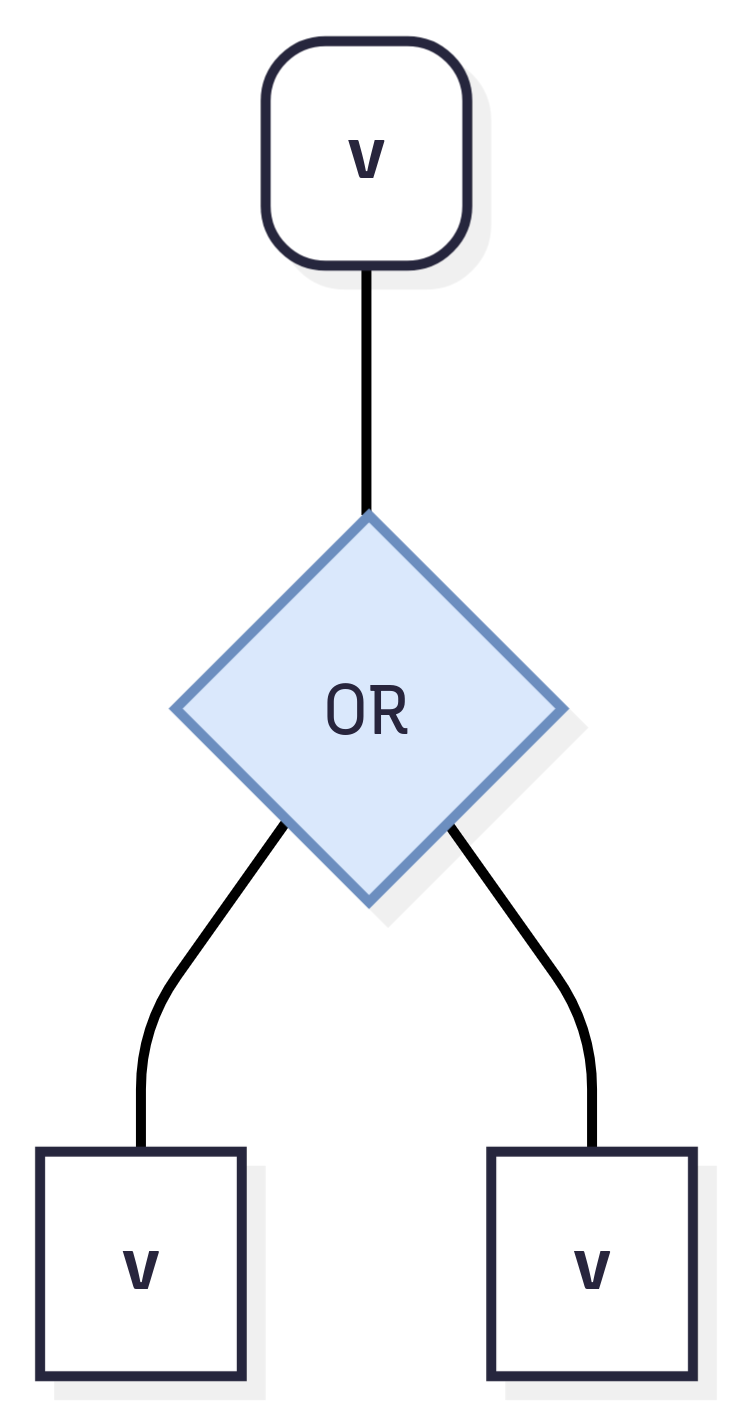
\includegraphics[width=0.2\textwidth]{images/or_gate.png}
    \hspace{0.05\textwidth}
    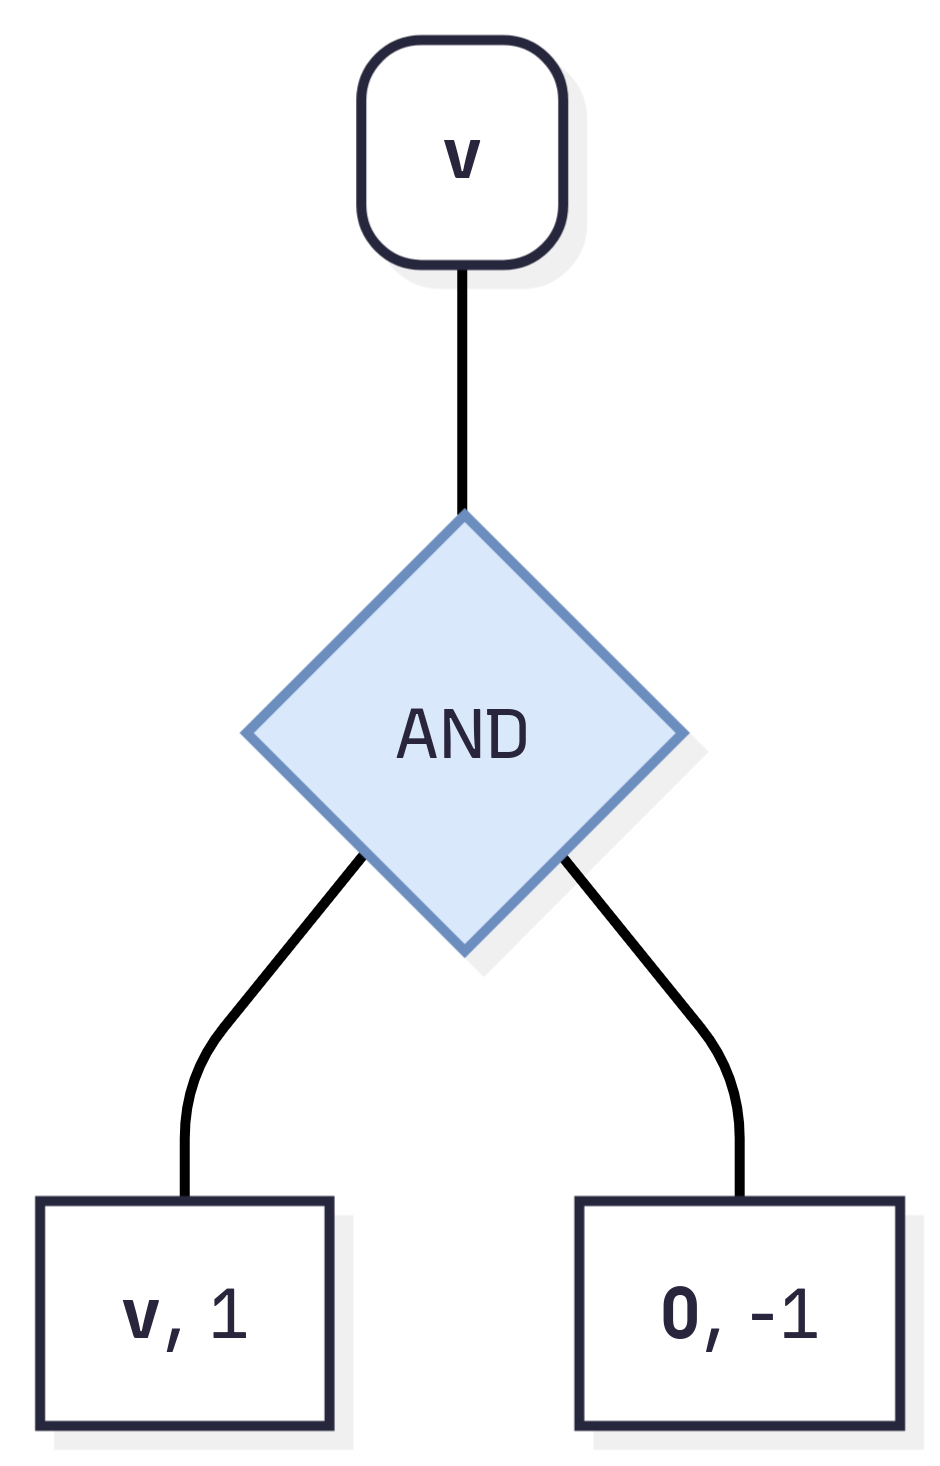
\includegraphics[width=0.2\textwidth]{images/and_gate.png}
    \caption{Porte OR e AND}
\end{figure}

Si parte dalla radice con il \emph{vettore target} $\mathbf{t}=(1,0,\dots,0)$ (prima coordinata associata al segreto $S$) e si applicano le regole fino alle foglie. I vettori alle foglie costituiscono le righe di $A$; un insieme di partecipanti è autorizzato se le sue righe generano $\mathbf{t}$.

\newpage

\begin{example}
    Riprendiamo l'esempio $P_1 \land (P_2 \lor (P_3 \land P_4))$ e costruiamo la matrice di accesso.

\begin{figure}[ht]
    \centering
    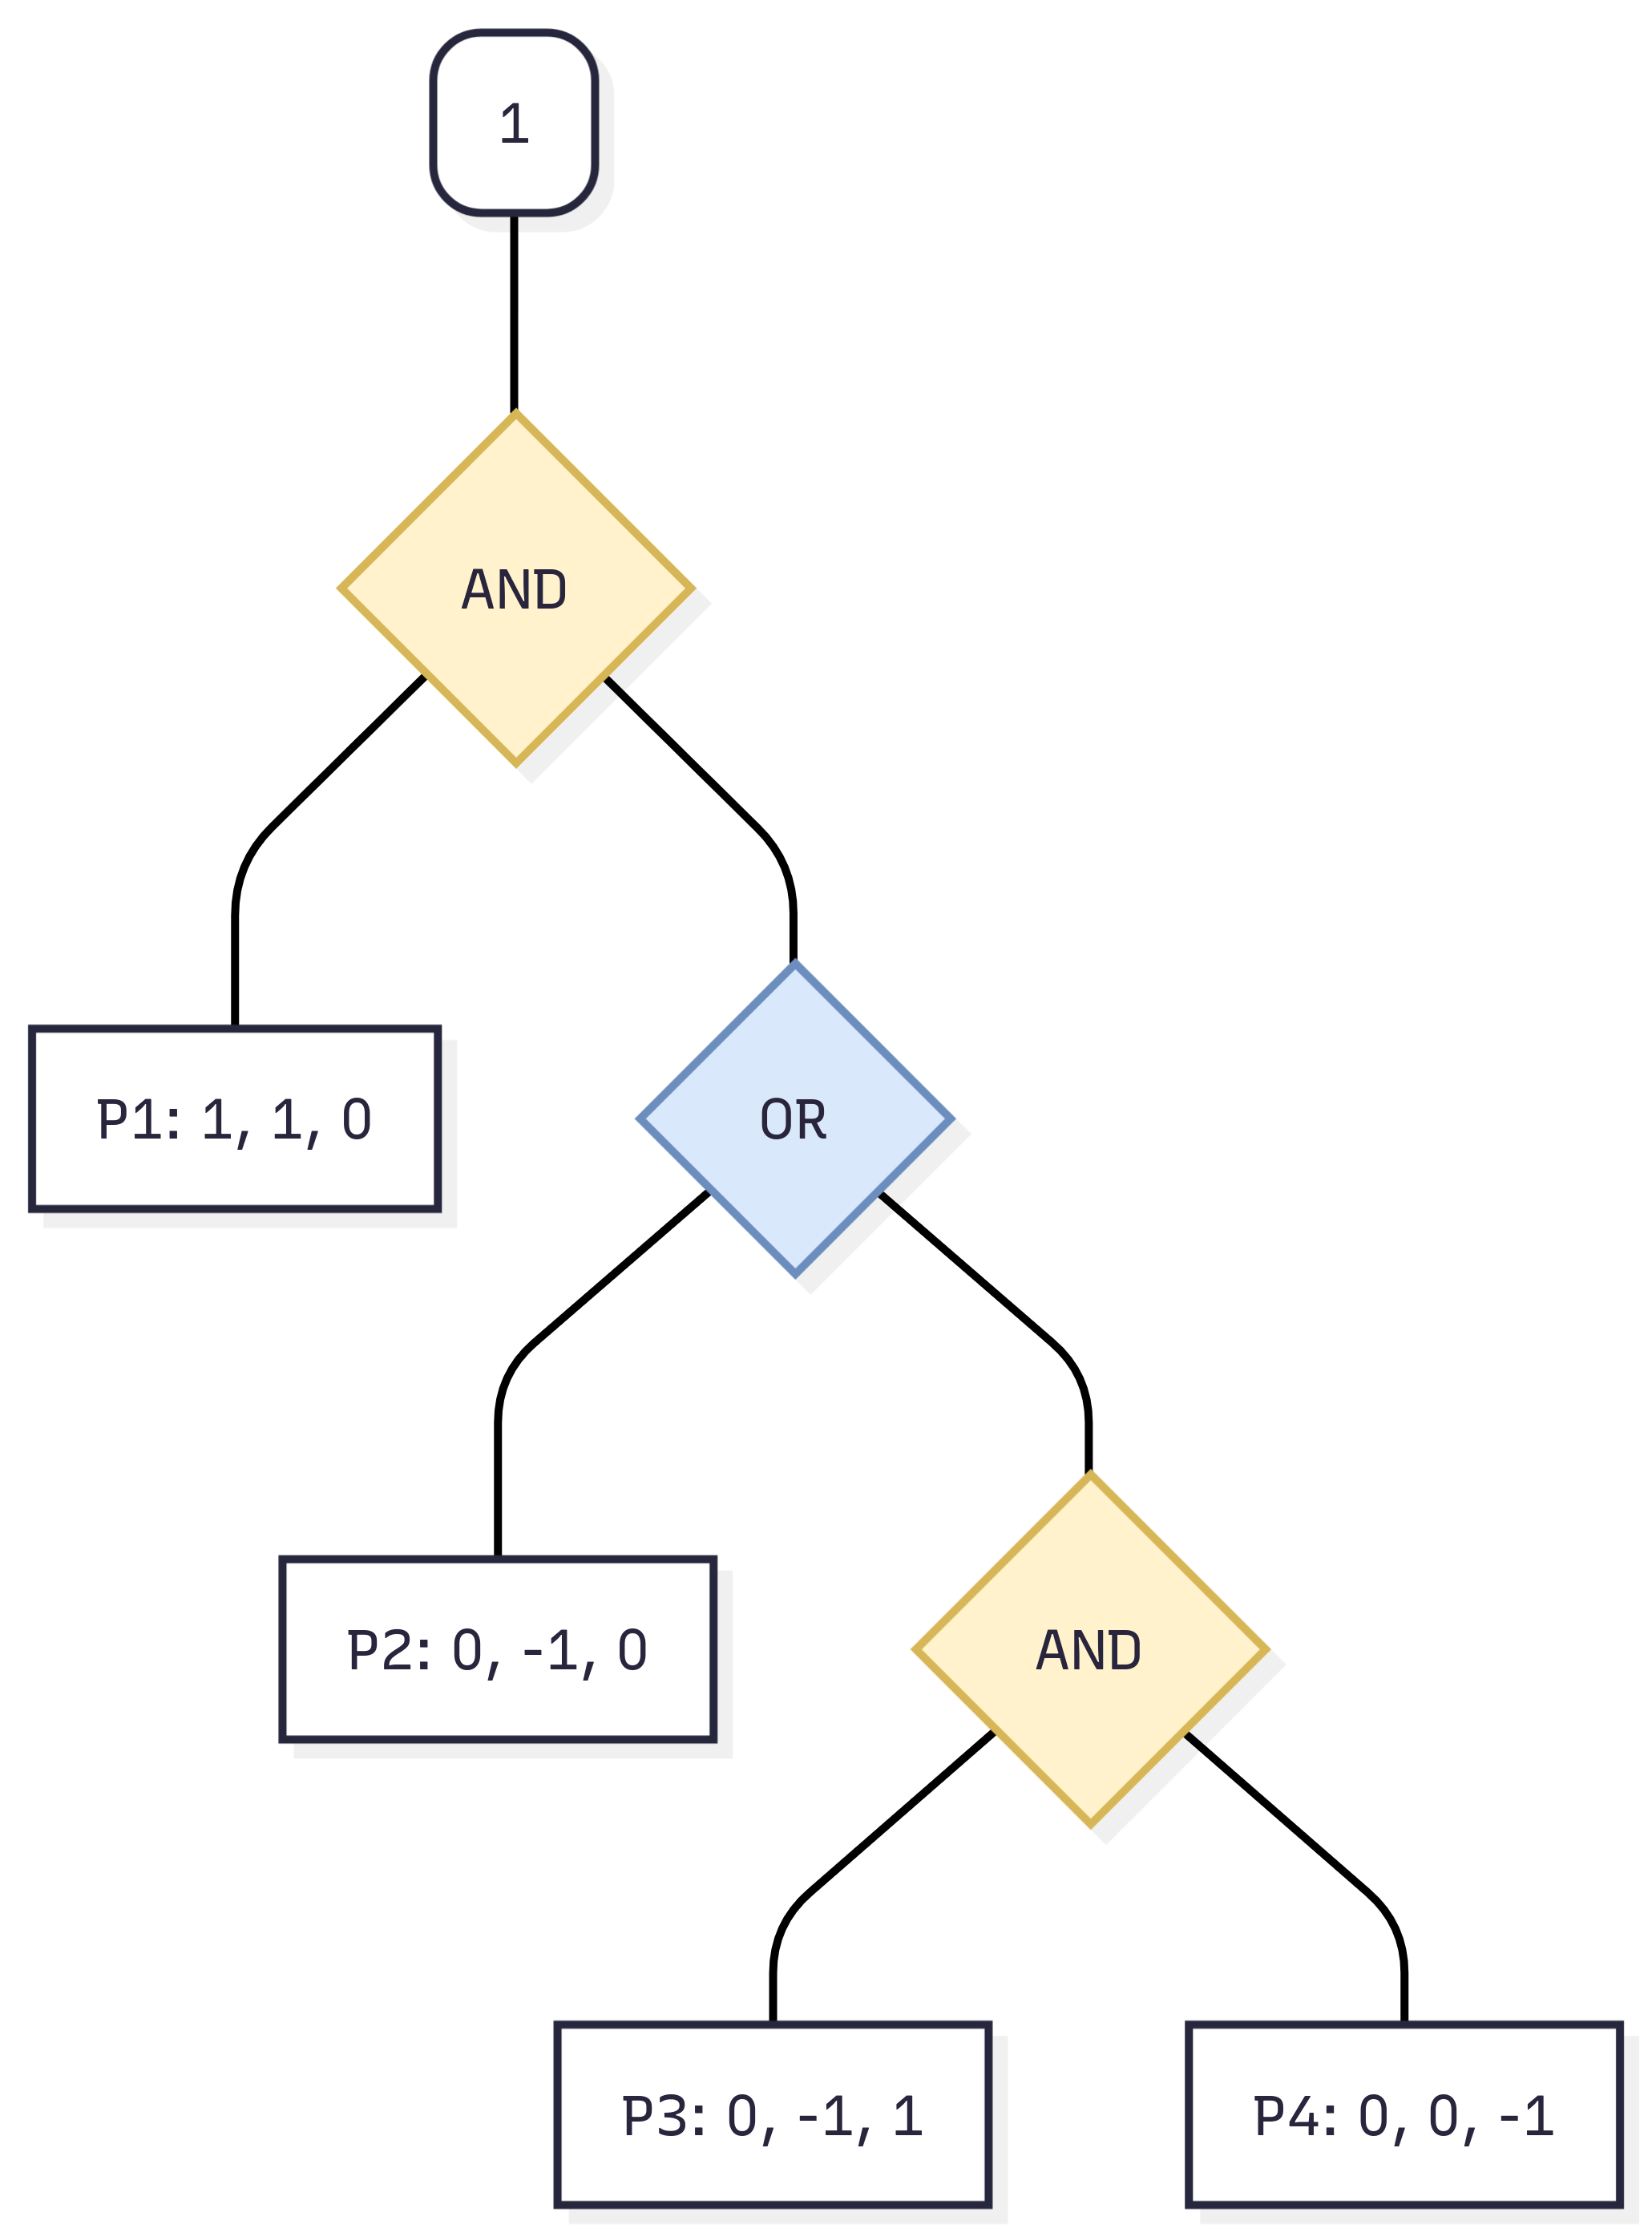
\includegraphics[width=0.4\textwidth]{images/example_or_and.png}
    \caption{Albero costruito a partire dalla formula logica.}
\end{figure}

Propagando il vettore target $\mathbf{t}=(1)$ e uniformando la dimensione a 3 si ottengono i vettori alle foglie:
\[
\begin{array}{c}
P_1\\ P_2\\ P_3\\ P_4
\end{array}
\left(
\begin{array}{ccc}
1 & 1 & 0\\
0 & -1 & 0\\
0 & -1 & 1\\
0 & 0 & -1
\end{array}
\right)=A,\qquad \mathbf{t}=(1,0,0).
\]

Condividendo $\mathbf{x}=(S,r_1,r_2)^T$, le quote sono
\[
y_1=S+r_1,\quad y_2=-r_1,\quad y_3=-r_1+r_2,\quad y_4=-r_2.
\]

Ricostruzione (insiemi minimali autorizzati):
\[
\{P_1,P_2\}:\ S=y_1+y_2,\qquad
\{P_1,P_3,P_4\}:\ S=y_1+y_3+y_4.
\]

\end{example}

\newpage

\section{Elliptic Curve}
La crittografia moderna fa ampio uso delle curve ellittiche per motivi di efficienza: a parità di sicurezza, le chiavi sono molto più piccole rispetto a RSA o agli schemi basati su $\mathbb{Z}_p^*$. Ad esempio, una chiave ECC da 256 bit è comparabile a una chiave RSA da 3072 bit; la crescita della sicurezza in ECC richiede chiavi di dimensione circa lineare, mentre in RSA è sostanzialmente esponenziale.

\begin{definition}[Curva ellittica]
    Sia $p>3$ un primo. Una curva ellittica $E_p(x, y)$ definita sul campo finito $\mathbb{F}_p$ è data (forma di Weierstrass ridotta) da
    \[
        y^2 \equiv x^3 + ax + b \pmod p,
    \]
    con $a,b \in \mathbb{F}_p$ tali che $4a^3 + 27b^2 \not\equiv 0 \pmod p$ (discriminante non nullo). Questa condizione garantisce che l'equazione $x^3 + ax + b = 0$ non ammetta doppia radice.
\end{definition}

L'insieme dei punti $E(\mathbb{F}_p)=\{(x,y)\in\mathbb{F}_p^2:\ y^2\equiv x^3+ax+b\} \cup \{\mathcal{O}\}$ forma un gruppo abeliano rispetto alla somma tra punti, dove $\mathcal{O}$ è il punto all'infinito (elemento neutro).

\begin{example}
    Consideriamo la curva $E_5(x, y)$ definita su $\mathbb{Z}_5$, dall'equazione
    \[
        y^2 = x^3 + x + 1
    \]
    Stiamo quindi considerando tutti quei punti
    \[
        E(\mathbb{Z}_5) 
        \{(x, y) \in \mathbb{Z}_5^2:\ y^2 \equiv x^3 + x + 1 \pmod 5\} \cup \{\mathcal{O}\} 
    \]

    \begin{description}
        \item[Elenco Quadrati: ] La prima cosa è enumerare i possibili valori di $y^2 \in \mathbb{Z}_5$.
        \[
        0^2 = 0, \quad 1^2 = 1, \quad 2^2 = 4, \quad 3^2 = 9 \pmod 5 \equiv 4, \quad 4^2 = 16 \pmod 5 \equiv 1
        \]
        I \textbf{residui quadratici sono quindi} $\{0, 1, 4\}$.
        \item[Calcolo Punti: ] Sostituiamo ogni possibile valore di $x \in \mathbb{Z_5}$ nell'equazione $y^2 = x^3 + x + 1 \pmod 5$:
        \begin{table}[h]
        \centering
        \renewcommand{\arraystretch}{1.5}
            \begin{tabular}{|c|l|c|c|l|}
            \hline
            \textbf{$x$} & \textbf{$y^2 = x^3 + x + 1 \pmod 5$} & \textbf{Quadrato?} & \textbf{$y$} & \textbf{Punti $(x, y)$} \\ \hline
            0 & $0 + 0 + 1 = 1$ & Sì & $1, 4$ & $(0, 1), (0, 4)$ \\ \hline
            1 & $1 + 1 + 1 = 3$ & No & - & - \\ \hline
            2 & $8 + 2 + 1 = 11 \equiv 1$ & Sì & $1, 4$ & $(2, 1), (2, 4)$ \\ \hline
            3 & $27 + 3 + 1 = 31 \equiv 1$ & Sì & $1, 4$ & $(3, 1), (3, 4)$ \\ \hline
            4 & $64 + 4 + 1 = 69 \equiv 4$ & Sì & $2, 3$ & $(4, 2), (4, 3)$ \\ \hline
            \multicolumn{5}{|c|}{\textbf{Punto all'infinito:} $\mathcal{O}$} \\ \hline
            \end{tabular}
        \caption{Ricerca dei punti della curva $E(\mathbb{Z}_5): y^2 = x^3 + x + 1$}
        \end{table}
    \end{description}
    \[
        E(\mathbb{Z}_5) = \{\mathcal{O}, (0, 1), (0, 4), (2, 1), (2, 4), (3, 1), (3, 4), (4, 2), (4, 3)\}
    \]
\end{example}

\begin{definition}[La legge di addizione]
Sia $E/\mathbb{F}_p$ (con $p>3$) definita da $y^2 \equiv x^3+ax+b \pmod{p}$.

Il punto all'infinito $\mathcal{O}$ è l'elemento neutro:
\[
    \forall P\in E(\mathbb{F}_p),\quad P+\mathcal{O}=\mathcal{O}+P=P.
\]

L'operazione di gruppo "$+$" sui punti di $E(\mathbb{F}_p)$ è definita come segue. Siano $P = (x_1, y_1)$ e $Q = (x_2, y_2)$ due punti, allora

\begin{description}
    \item[Se $\mathbf{x_1 \neq x_2}$:] Ponendo $\lambda \equiv (y_2-y_1)(x_2-x_1)^{-1} \pmod p$, si ha
    \[
        x_3 \equiv \lambda^2 - x_1 - x_2 \pmod p, 
        \qquad 
        y_3 \equiv \lambda(x_1 - x_3) - y_1 \pmod p.
    \]
    Allora $P + Q = R = (x_3, y_3)$.
    \item[Se $\mathbf{P=Q=(x_1,y_1)\ \text{con}\ y_1\neq 0}$:] Ponendo $\lambda \equiv (3x_1^2 + a)(2y_1)^{-1} \pmod p$, si ha
    \[
        x_3 \equiv \lambda^2 - 2x_1 \pmod p, 
        \qquad 
        y_3 \equiv \lambda(x_1 - x_3) - y_1 \pmod p.
    \]
    Allora $2P = R = (x_3, y_3)$.
    \item[Se $\mathbf{x_1=x_2}$ e $\mathbf{y_1 \equiv -y_2 \pmod p}$:] $P+Q=\mathcal{O}$.
    \item[Se $\mathbf{P=Q}$ e $\mathbf{y_1=0}$:] $2P=\mathcal{O}$.
\end{description}
\end{definition}
Questa legge di addizione rende l'insieme $E(\mathbb{F}_p)$ un gruppo. L'elemento identità è il punto all'infinito $\mathcal{O}$. Ogni punto $P=(x_1,y_1)\in E(\mathbb{F}_p)$, con $P\neq\mathcal{O}$, ha inverso additivo $-P=(x_1,-y_1)$. Inoltre si può dimostrare che la legge è associativa. La legge è chiaramente commutativa, $P+Q=Q+P$ per tutti $P,Q\in E(\mathbb{F}_p)$, rendendo il gruppo \textbf{abeliano}.
Come in ogni gruppo, per un punto $P\in E(\mathbb{F}_p)$ si scrive $2P:=P+P$, $3P:=P+P+P$ e, più in generale, $\alpha P := (\alpha-1)P + P$ per ogni intero positivo $\alpha$. Si noti che $\alpha P$ può essere calcolato con al più $2\log_2\alpha$ operazioni di gruppo usando l'algoritmo di raddoppio e somma (double-and-add).

\begin{example}
    Consideriamo i seguenti due punti $P = (0, 1) \in E=(\mathbb{Z}_5)$ e $Q = (0, 1) \in E=(\mathbb{Z}_5)$, dove $E_5(x, y): y^2 = x^3 + x + 1$
    
    Osserviamo che $P = Q$ quindi ci troviamo nel secondo caso, di conseguenza:
    \begin{align*}
        \lambda &= (3x_1^2 + a)(2y_1)^{-1} \pmod 5 = 1 \cdot 2^{-1} \pmod 5 = 1 \cdot 3 = 3 \\
        x_3 &= \lambda^2 -2x_1 \pmod 5 = 3^2 \pmod 5 = 4 \\
        y_3 &= \lambda(x_1 - x_3) - y_1 \pmod 5 = 3(0 - 4) - 1 \pmod 5 = 3 - 1 = 2
    \end{align*}
    $P + Q = 2P = (4, 2)$
\end{example}
\begin{example}
    Consideriamo i seguenti due punti $P = (4, 2) \in E=(\mathbb{Z}_5)$ e $Q = (0, 1) \in E=(\mathbb{Z}_5)$, dove $E_5(x, y): y^2 = x^3 + x + 1$
    
    Osserviamo che $P \neq Q$ quindi ci troviamo nel primo caso, di conseguenza:
    \begin{align*}
        \lambda &= (y_2 - y_1)(x_2 - x_1)^{-1} \pmod 5 = -1 \cdot -4^{-1} \pmod 5 = 4 \cdot 1 = 4 \\
        x_3 &= \lambda^2 -x_1 -x_2 \pmod 5 = 4^2 - 4 \pmod 5 = 12 \pmod 5 = 2 \\
        y_3 &= \lambda(x_1 - x_3) - y_1 \pmod 5 = 4(2) - 2 \pmod 5 = 1
    \end{align*}
    $P + Q = (2, 1)$
\end{example}

\subsection{EC Group for Cryptography}

Si consideri una curva ellittica $E/\mathbb{F}_p$ e il gruppo $E(\mathbb{F}_p)$ dei punti definiti su $\mathbb{F}_p$. È noto che $E(\mathbb{F}_p)$ è un gruppo abeliano finito; supponiamo inoltre che sia ciclico, ossia generato da un punto $P \in E(\mathbb{F}_p)$. Possiamo allora analizzare la difficoltà di problemi come il logaritmo discreto, il Diffie-Hellman computazionale (CDH) e il Diffie-Hellman decisionale (DDH) nel gruppo $E(\mathbb{F}_p)$. Quando tali problemi risultano difficili in $E(\mathbb{F}_p)$, tutte le costruzioni crittografiche viste in precedenza possono essere instanziate in questo gruppo, ottenendo sistemi su curve ellittiche.

\begin{definition}[ECDLP]
    Sia $P$ un punto di ordine $q$ (cioè $qP=\mathcal{O}$). Dati $P$ e $q$, insieme a un punto $Q:=\alpha P$ per qualche $\alpha \in \mathbb{Z}_q$, si chiede di determinare $\alpha$. Qui $\alpha P$ indica il punto ottenuto sommando $P$ a sé stesso $\alpha$ volte secondo la legge di addizione del gruppo.
\end{definition}

La scelta della curva è cruciale sia per la sicurezza sia per l'efficienza. È preferibile adottare curve raccomandate dagli standard (NIST/SECG, CFRG) e ricordare che non si lavora solo su campi primi $\mathbb{F}_p$, ma anche su campi binari $\mathbb{F}_{2^m}$. Le curve moderne, come le Edwards e le Montgomery, impiegano forme diverse dalla Weierstrass e tendono a essere più efficienti e robuste. Ogni famiglia di curve presenta proprietà e assunzioni differenti (ordine del gruppo, cofattore, \emph{pairing-friendliness}, ipotesi DL/CDH/DDH), con effetti concreti sui protocolli che vi si basano. In particolare, nelle famiglie con mappe bilineari il problema decisionale di Diffie-Hellman (DDH) può risultare facile mentre quello computazionale (CDH) resta difficile; per questo la selezione della curva va allineata alle garanzie richieste dal protocollo.

Consideriamo la moltiplicazione per scalare (analoga all'esponenziazione modulare). In un gruppo di ordine di circa 160 bit, cioè $q \approx 2^{160}$, il costo computazionale è $O(\log q)$: con l'algoritmo \textit{double-and-add} (analogo di \textit{square-and-multiply}) servono in media $\approx \tfrac{3}{2}\log_2 q$ operazioni di gruppo (raddoppi e somme).

\subsection{Algoritmio Double-and-Add}

Dato un punto $P$ su una curva ellittica e un intero $k\ge 0$, la moltiplicazione scalare $kP$ si ottiene combinando ripetutamente le operazioni di raddoppio ($2Q$) e somma ($Q+R$).

\begin{tcolorbox}[title=Double-and-Add (da sinistra a destra), colback=green!5, colframe=green!50!black]
Input: $k=(b_{\ell-1}\dots b_1b_0)_2$, $P$; Output: $Q=kP$.
\begin{enumerate}[leftmargin=*]
    \item $Q\leftarrow \mathcal{O}$
    \item Per $i=\ell-1,\dots,0$:
        \begin{enumerate}[leftmargin=*]
            \item $Q\leftarrow 2Q$
            \item Se $b_i=1$ allora $Q\leftarrow Q+P$
        \end{enumerate}
    \item Restituisci $Q$
\end{enumerate}
Costo: $\ell$ raddoppi e $\mathrm{wt}(k)$ somme, dove $\mathrm{wt}(k)$ è il numero di bit a 1. In media, per $k$ casuale, si hanno $\approx \ell$ raddoppi e $\approx \ell/2$ somme.
\end{tcolorbox}

\begin{example}
    Supponiamo di voler calcolare $[1437]P$. Innanzitutto esprimiamo in bits 1437.
    \[
        (1437)_{10} = (10110011101)_2
    \]

    La regola di lettura standard è da $LSB \to MSB$.
    Inizializziamo $R = \mathcal{O}$
    \begin{center}
        \begin{tabular}{ |c|c|c| } 
        \hline
        $\mathbf{LSB \to MSB}$ & \textbf{Double} & \textbf{Result} \\ 
        \hline
        1 & $1P$ & $R = R + P$ \\
        \hline
        0 & $2P$ & - \\
        \hline
        1 & $4P$ & $R = R + 4P = 5P$ \\
        \hline
        1 & $8P$ & $R = R + 8P = 13P$ \\
        \hline
        1 & $16P$ & $R = R + 16P = 29P$ \\
        \hline
        0 & $32P$ & - \\
        \hline
        0 & $64P$ & - \\
        \hline
        1 & $128P$ & $R = R + 128P = 157P$ \\
        \hline
        1 & $256P$ & $R = R + 256P = 413P$ \\
        \hline
        0 & $512P$ & - \\
        \hline
        1 & $1024P$ & $R = R + 1024P = 1437P$ \\
        \hline    
        \end{tabular}
    \end{center}
\end{example}

\paragraph{Sicurezza}
La sicurezza delle operazioni su curve ellittiche si basa su problemi considerati difficili:
\begin{itemize}
    \item Dato un punto generatore $P$ e un punto $Q=[k]P$, risalire allo scalare $k$ è computazionalmente difficile. Questo è il \textbf{Problema del Logaritmo Discreto su Curve Ellittiche (ECDLP)}.
    \item In molte curve si assumono difficili anche:
        \begin{description}
            \item[Computational Diffie-Hellman (CDH):] dati $P$, $[a]P$, $[b]P$, calcolare $[ab]P$;
            \item[Decisional Diffie-Hellman (DDH):] distinguere 
            \[
            (P,\ [a]P,\ [b]P,\ [ab]P) \text{ da } (P,\ [a]P,\ [b]P,\ [c]P)
            \]
            con $c$ casuale.
        \end{description}
\end{itemize}

\subsection{ECDH}

L'obiettivo di ECDH è permettere a due parti (Alex A e Bob B) di stabilire un segreto condiviso su un canale pubblico, senza rivelare le chiavi private.

\paragraph{Parametri comuni (setup)}
Si fissano i parametri di dominio
\[
\mathsf{DP}=(p,a,b,G,q),
\]
dove:
\begin{itemize}[leftmargin=*]
    \item $E/\mathbb{F}_p$: $y^2 \equiv x^3 + ax + b \pmod p$ con discriminante non nullo;
    \item $G\in E(\mathbb{F}_p)$ è un generatore di ordine primo $q$;
\end{itemize}

\paragraph{Protocollo}
\begin{enumerate}[itemsep=2pt, topsep=2pt]
    \item Generazione delle chiavi:
    \[
        x\gets_{u.a.r.}\mathbb{Z}_q^*,\quad X=[x]G
        \qquad\text{e}\qquad
        y\gets_{u.a.r.}\mathbb{Z}_q^*,\quad Y=[y]G.
    \]
    C invia $X$ a B, B invia $Y$ a A.
    \item Calcolo del segreto condiviso:
    \[
        S_A=[x]Y=[x]([y]G)=[xy]G,\qquad
        S_B=[y]X=[y]([x]G)=[xy]G.
    \]
    Entrambe le parti ottengono lo stesso punto $S=[xy]G$.
    \item Derivazione della chiave:
    \[
        k=\mathrm{KDF}\big(\mathrm{enc}(S)\big)\ \ \text{(es. usando la coordinata }x\text{ di }S\text{ e un salt)}.
    \]
\end{enumerate}
\paragraph{Note operative}
\begin{itemize}
    \item Validare le chiavi pubbliche ricevute: $P\neq\mathcal{O}$, coordinate in $\mathbb{F}_p$, $P$ sulla curva e nel sottogruppo di ordine $q$ (ad es. verificando $[q]P=\mathcal{O}$).
    \item Usare chiavi effimere (ECDHE) per la Perfect Forward Secrecy: generare coppie fresh per sessione e autenticare le chiavi pubbliche per evitare MITM.
    \item Non usare direttamente il punto $S$ come chiave: derivare sempre le chiavi con una KDF (es. HKDF) con salt/label e contesto (transcript, identità).
\end{itemize}

\subsection{ECDSA}

L'ECDSA (Elliptic Curve Digital Signature Algorithm) fornisce autenticità e integrità su gruppi di punti ellittici ed è basato sulla difficoltà dell'ECDLP.

\paragraph{Parametri e chiavi}
\begin{itemize}[itemsep=2pt, topsep=2pt]
    \item Parametri di dominio $\mathsf{DP}=(p,a,b,G,q)$ su $E/\mathbb{F}_p$, con $G\in E(\mathbb{F}_p)$ generatore di ordine primo $q$.
    \item Funzione di hash $H:\{0,1\}^*\to\{0,1\}^*$ e digest ridotto $(H(m))$.
    \item Chiave privata: $d\in\{1,\dots,q-1\}$.
    \item Chiave pubblica: $Q=[d]G$.
\end{itemize}

Firma di un messaggio $m$
\begin{enumerate}[itemsep=2pt, topsep=2pt]
    \item Calcola $(H(m))$.
    \item Scegli $k\gets_{u.a.r.}\{1,\dots,q-1\}$ (nonce unico e segreto).
    \item Poni $R=[k]G=(x_1,y_1)$ e $r=x_1 \bmod q$; se $r=0$ ripeti dal punto 2.
    \item Calcola $s=k^{-1}(H(m) + d\,r)\bmod q$; se $s=0$ ripeti dal punto 2.
    \item La firma è la coppia $(r,s)$.
\end{enumerate}

Verifica di $(r,s)$ su $m$ con $Q$
\begin{enumerate}[itemsep=2pt, topsep=2pt]
    \item Rifiuta se $r\notin\{1,\dots,q-1\}$ o $s\notin\{1,\dots,q-1\}$.
    \item Calcola $H(m)$ e $w=s^{-1}\bmod q$.
    \item Poni $u_1=H(m)\,w \bmod q$, $u_2=r\,w \bmod q$.
    \item Calcola $X=[u_1]G+[u_2]Q=(x_0,y_0)$; se $X=\mathcal{O}$ rifiuta.
    \[
    \begin{aligned}
    X &= [u_1]G+[u_2]Q \\
        &= [H(m)w]G + [rw]Q \\
        &= [H(m)s^{-1}]G + [rs^{-1}]Q \\
        &= [H(m)s^{-1}]G + [rs^{-1}d]G \\
        &= [(H(m)+rd)s^{-1}]G \\
        &= [k]G = R,
    \end{aligned}
    \]
    dove $s \equiv k^{-1}(H(m)+rd) \pmod q$ implica $(H(m)+rd)s^{-1}\equiv k \pmod q$.

    \item Accetta se $x_0 \bmod q = r$, altrimenti rifiuta.
\end{enumerate}

\paragraph{Note operative}
\begin{itemize}
    \item Nonce $k$: deve essere unico e imprevedibile; è consigliato utilizzare RFC 6979 per un nonce deterministico. \textbf{Non deve essere mai divulgato!}
    \item Validazione di $Q$: verifica che $Q\neq\mathcal{O}$, che $Q\in E(\mathbb{F}_p)$ e che $[q]Q=\mathcal{O}$.
\end{itemize}

\begin{description}
    \item[Cosa accade se $\mathbf{k}$ è prevedibile?] In ECDSA la sicurezza richiede che $k$ sia un nonce segreto, unico e imprevedibile per ogni firma. Se un avversario conosce $k$, da $(r,s)$ e $H(m)$ ricava subito la chiave privata:
    \[
    s \equiv k^{-1}(H(m)+r\,d) \ \Rightarrow\ sk \equiv H(m)+r\,d \ \Rightarrow\ d \equiv (sk - H(m))\,r^{-1} \pmod q.
    \]

    \item[Cosa accade se $\mathbf{k}$ viene riutilizzato?] Firmando due messaggi diversi $m_1,m_2$ con lo stesso $k$ si ottiene lo stesso $r$ e si può recuperare $k$ (e quindi $d$) anche senza conoscerlo a priori. Ponendo $z_i=H(m_i)$:
    \[
    \begin{aligned}
    s_1 &\equiv k^{-1}(z_1 + r\,d) \pmod q,\\
    s_2 &\equiv k^{-1}(z_2 + r\,d) \pmod q,
    \end{aligned}
    \]
    sottraendo:
    \[
    s_1 - s_2 \equiv k^{-1}(z_1 - z_2) \pmod q
    \ \Rightarrow\
    k \equiv (z_1 - z_2)\,(s_1 - s_2)^{-1} \pmod q.
    \]
    Infine:
    \[
    d \equiv (s_1\,k - z_1)\,r^{-1} \pmod q.
    \]
    Quindi il riuso di $k$ compromette la chiave privata.
\end{description}

\newpage

\section{Bilinear Maps}

Una mappa bilineare (o pairing), indicata di solito con $e$, è una funzione che collega due gruppi crittografici $G_1$ e $G_2$ producendo un elemento in un terzo gruppo $G_T$.

\begin{definition}[Mappa bilineare]
Siano $G_1,\ G_2,\ G_T$ gruppi ciclici di ordine primo $q$, con generatori $g_1\in G_1$ e $g_2\in G_2$. Una funzione
\[
e:\ G_1\times G_2 \to G_T
\]
è detta una mappa bilineare se soddisfa:
\begin{enumerate}[itemsep=2pt, topsep=2pt]
    \item \textbf{Bilinearità:} per ogni $u\in G_1$, $v\in G_2$ e $a,b\in\mathbb{Z}_q$,
    \[
        e(u^a, v^b)=e(u,v)^{ab}.
    \]
    \item \textbf{Non-degenerazione:} $e(g_1,g_2)\neq 1_{G_T}$ (equivalentemente, $e(g_1,g_2)$ genera $G_T$).
    \item \textbf{Computabilità efficiente:} $e$ è calcolabile in tempo polinomiale.
\end{enumerate}
\end{definition}

\textbf{Nota}
Se usiamo la notazione additiva tipica delle curve ellittiche, la formula diventa $e([a]P,\ [b]Q)=e(P, Q)^{ab}$

Dalla bilinearità seguono le identità:
\[
    e(u_1u_2,v) = e(u_1,v) \cdot e(u_2,v), \qquad e(u,v_1v_2) = e(u,v_1) \cdot e(u,v_2)
\]

\begin{example}
    Semplificazione dell'espressione utilizzando le proprietà delle mappe bilineari:
    \begin{align*}
        e(ag^b, g^{c+d}) 
        &= e(g^{ab}, g^{c+d}) && \text{(Moltiplicazione scalare come esponente: } ag^b \to g^{ab}\text{)} \\
        &= e(g^{ab}, g^c \cdot g^d) \\
        &\overbrace{=}^{\text{linearità}} e(g^{ab}, g^c) \cdot e(g^{ab}, g^d) && \text{(Distribuzione sul secondo argomento)} \\
        &\overbrace{=}^{\text{bilinearità}} e(g, g)^{abc} \cdot e(g, g)^{abd} && \text{(Estrazione degli esponenti in } G_t\text{)} \\
        &= e(g, g)^{abc + abd} \\
        &= g_t^{ab(c+d)} 
    \end{align*}
\end{example}

Nel caso $G_1=G_2$ si parla di pairing simmetrico; altrimenti è asimmetrico.

Da ora in poi supponiamo sempre che $G = G_1 = G_2$.


In pratica, il gruppo $G$ è scelto quasi sempre come l'insieme dei punti di una curva ellittica (o di un suo sottogruppo) definita su un campo finito. Un esempio elementare è la curva
$y^2 = x^3 + 1$
su $\mathbb{F}_p$, che fornisce un gruppo abeliano efficiente su cui definire la mappa bilineare.

Più in generale, $G$ può essere visto come una varietà abeliana su un campo: le curve ellittiche ne sono il caso di dimensione 1, ma sono state studiate anche varietà abeliane di dimensione superiore per ottenere pairing con proprietà specifiche.

Il gruppo di arrivo $G_T$ è tipicamente il gruppo moltiplicativo di un campo finito; è qui che vive l'output del pairing e dove si sfruttano le identità indotte dalla bilinearità.

\subsection{Decisional Diffie-Hellman}

Un primo problema affrontabile con le mappe bilineari è il \textit{Decisional Diffie-Hellman (DDH)}.

\begin{definition}[DDH]
    Sia $G$ un gruppo ciclico di ordine primo $q$ con generatore $g$. Il vantaggio di un algoritmo probabilistico $\mathcal{A}$ nel distinguere una tupla Diffie–Hellman valida da una casuale è
    \[
    \text{Adv}^{\mathrm{DDH}}_{\mathcal{A},G}
    =
    \left|
      \Pr\!\big[\mathcal{A}(g, g^a, g^b, g^{ab}) = 1\big]
      - 
      \Pr\!\big[\mathcal{A}(g, g^a, g^b, g^{z}) = 1\big]
    \right|,
    \]
    dove $a,b,z \gets_{u.a.r.} \mathbb{Z}_q$.
\end{definition}

Se l'Advantage è \textbf{vicino a 0}, l'algoritmo sta praticamente tirando a indovinare; quindi il DDH è \text{difficile} (buono per la sicurezza classica).

Se l'Advantage è \textbf{vicino a 1}, l'algoritmo distingue perfettamente i due casi; quindi il DDH è \textbf{facile}.

In un gruppo crittografico standard, distinguere una quaterna di Diffie-Hellman $(g, g^a, g^b, g^{ab})$ da una quaterna casuale $(g, g^a, g^b, g^z)$ è ritenuto impossibile per un computer in tempi ragionevoli. Tuttavia, se disponiamo di una mappa bilineare $e:G \times G \to G_t$, un algoritmo può risolvere questo problema in tempo polinomiale.

Con una mappa bilineare $e:G\times G\to G_T$, DDH diventa facile: dato $(g, g^a, g^b, g^z)$, si verifica
\[
e(g^a, g^b) \overset{?}{=} e(g, g^z).
\]
Grazie alla proprietà di bilinearità, sappiamo che $e(g^a, g^b) = e(g,g)^{ab}$. Se $z = ab$, allora anche $e(g, g^z) = e(g,g)^{ab}$. Se i due risultati coincidono, la quaterna è valida.

\begin{example}
    Immagina di ricevere quattro valori e di voler verificare se formano una quaterna di Diffie–Hellman valida \((P,\,[2]P,\,[3]P,\,[6]P)\) con \([6]P=[2\cdot 3]P\).

    Test con la mappa bilineare. Poni \(Z=e(P,P)\in G_T\). Allora:
    \[
        e([2]P,[3]P)=e(P,P)^{2\cdot 3}=Z^{6},
        \qquad
        e(P,[6]P)=e(P,P)^{6}=Z^{6}.
    \]
    Poiché i due risultati coincidono, la quaterna è valida.

    Se invece l'ultimo valore fosse \([7]P\), avremmo
    \[
        e(P,[7]P)=e(P,P)^{7}=Z^{7}\neq Z^{6},
    \]
    e la quaterna non sarebbe valida.
\end{example}

\subsubsection*{Nota su Computationl Diffie-Hellman (CDH)}

È utile sottolineare che il problema computazionale di Diffie-Hellman (CDH) può rimanere difficile in un gruppo ciclico $G$ anche quando il problema decisionale (DDH) è facile, ad esempio grazie alla disponibilità di una mappa bilineare. Non è infatti noto, in generale, come usare un pairing per risolvere CDH. Si definisce \emph{gap Diffie-Hellman} (GDH) un gruppo di ordine primo in cui DDH è facile ma CDH resta difficile; questa definizione non dipende dall'esistenza di una mappa bilineare. Le mappe bilineari si possono quindi interpretare come uno strumento per ottenere (o modellare) gruppi con tale “gap”: rendono semplice distinguere le tuple di Diffie-Hellman valide (DDH), senza offrire un metodo efficiente per calcolare $[ab]P$ a partire da $[a]P$ e $[b]P$ (CDH).

\subsubsection*{Logaritmo Discreto}

\begin{theorem}
    Se esiste una mappa bilineare $e: G \times G \to G_T$, allora il problema del logaritmo discreto in $G$ non è più difficile del problema del logaritmo discreto in $G_T$ (riduzione in tempo polinomiale).
\end{theorem}

Dati $g\in G$ e $g^a\in G$, si calcolano $e(g,g)\in G_T$ ed $e(g,g^a)=e(g,g)^a\in G_T$. A questo punto si applica un risolutore del logaritmo discreto in $G_T$ per ricavare $a$. Questa procedura è nota come riduzione di Menezes--Okamoto--Vanstone (MOV).

\subsection{Joux's 3-Party Diffie-Hellman}

Sia $G$ un gruppo ciclico di ordine primo $q$, $e: G \times G \to G_T$ una mappa bilineare, e $g$ un generatore di $G$. Poni $\hat{g} = e(g,g) \in G_T$.

\textbf{Protocollo.}
\begin{enumerate}[itemsep=2pt, topsep=2pt]
    \item Alice, Bob e Carol scelgono $a,b,c \gets_{u.a.r.}\mathbb{Z}_q$.
    \item Trasmettono pubblicamente $g^a,\ g^b,\ g^c$.
    \item Calcolo del segreto condiviso (uguale per tutti grazie alla bilinearità):
    \[
        \text{Alice: } e(g^b,g^c)^a=\hat{g}^{abc},\quad
        \text{Bob: } e(g^c,g^a)^b=\hat{g}^{abc},\quad
        \text{Carol: } e(g^a,g^b)^c=\hat{g}^{abc}.
    \]
\end{enumerate}
La chiave finale si deriva come $k=\mathrm{KDF}\big(\mathrm{enc}(\hat{g}^{abc})\big)$.

Dal punto di vista di Alice, la mappa bilineare consente un "trucco" per ottenere \(\hat{g}^{\,bc}\) a partire da \(g^b\) e \(g^c\):
\[
e(g^b,g^c)=e(g,g)^{bc}=\hat{g}^{\,bc}.
\]
Poi una normale esponenziazione porta a \(\hat{g}^{\,abc}\):
\[
(\hat{g}^{\,bc})^{a}=\hat{g}^{\,abc}.
\]
Non è possibile usare \(e\) in modo annidato per ottenere direttamente \(\hat{g}^{\,abc}\) da \(g^a, g^b, g^c\), perché il secondo argomento di \(e\) deve appartenere a \(G\):
\[
e\big(g^a,\, e(g^b,g^c)\big) = e(g^a, \hat{g}^{bc}) \neq \hat{g}^{abc} \quad \text{poiché } \hat{g}^{bc} \notin G
\]
In sintesi, è consentita una \textbf{sola applicazione} del pairing.

\subsection{Boneh and Franklin's IBE Scheme}

\begin{definition}[Identity-Based Encryption (IBE) di Boneh.Franklin]
L'idea è cifrare direttamente verso un'identità testuale (es. un'email) usata come chiave pubblica, eliminando certificati e gestione PKI. Un'autorità fidata (PKG - Private Key Generator) detiene una \textit{master key} e, su richiesta, estrae la chiave privata associata all'identità. Lo schema di Boneh-Franklin realizza IBE usando mappe bilineari: la sicurezza si basa sulla difficoltà di Diffie-Hellman bilineare (BDH) e sull-uso di funzioni di hash in modello random oracle.
\end{definition}

Sia $G$ un gruppo ciclico di ordine primo $q$, $e: G \times G \to G_T$ una mappa bilineare, e $g$ un generatore di $G$. Poni $\hat{g}=e(g,g)\in G_T$. Siano $h_1:\{0,1\}^\ast \to G$ e $h_2:G_T \to \{0,1\}^\ast$ funzioni di hash. Tutti questi sono parametri pubblici.

\begin{description}
    \item[SETUP:] La PKG estrare $s \gets_{u.a.r.} \in \mathbb{Z}_q$ e calcola la chiave pubblica $g^s$.
    \item[CIFRATURA:] Alice vuole inviare un messaggio $m$ a Bob. Estrae $r \gets_{u.a.r.} \in \mathbb{Z}_q$ e calcola:
    \begin{align*}
        ENC(g,\ g^s,\ \text{"Bob"},\ m) 
        &= \left( g^r, m \oplus h_2(e(h_1(\text{"Bob"}),\ g^s)^r) \right) \\
        &= \left( g^r, m \oplus h_2(e(h_1(\text{"Bob"}),\ g)^{sr}) \right)
    \end{align*}
    \item[GENERAZIONE PK:] Ora, la PKG crea la chiave privata di Bob nel seguente modo:
    \[
        \texttt{MakeKey}(s, \text{"Bob"}) = h_1(\text{"Bob"})^s
    \]
    \item[DECIFRATURA:] Ricevuto il messaggio cifrato $(u, v) = \left( g^r, m \oplus h_2(e(h_1(\text{"Bob"}),\ g)^{sr}) \right)$, usa la chiave privata $w = h_1(\text{"Bob"})^s$, Bob decifra nel seguente modo:
    \begin{align*}
        DEC(u, v, w) &= v \oplus h_2(e(w, u)) \\
        &= m \oplus h_2(e(h_1(\text{"Bob"}),\ g)^{sr}) \oplus h_2(e(h_1(\text{"Bob"})^s,\ g^r)) \\
        &= m \oplus h_2(e(h_1(\text{"Bob"}),\ g)^{sr}) \oplus h_2(e(h_1(\text{"Bob"}),\ g)^{sr}) \\
        &= m
    \end{align*}
\end{description}

Pensiamo a tre attori che cooperano per derivare una chiave condivisa.
Alice (mittente) sceglie $r$ e pubblica $u=g^{r}$.
La PKG (autorità) possiede il segreto $s$ e pubblica $g^{s}$.
Bob (destinatario) ha come "chiave pubblica" $h_1(\text{"Bob"})\in G$, che si può immaginare come $h_1(\text{"Bob"})=g^{t}$ con $t$ ignoto.
L'obiettivo è ottenere $\hat{g}^{\,rst}$, dove $\hat{g}=e(g,g)$, da usare come chiave di sessione.

Come Bob ottiene la chiave.
Bob non conosce $t$, quindi la PKG gli fornisce in modo sicuro la chiave privata
$w=h_1(\text{"Bob"})^{s}=g^{st}$.
Avendo $u=g^{r}$ dal cifrato di Alice, Bob calcola
\[
e(w,u)=e(g^{st},g^{r})=e(g,g)^{\,rst}=\hat{g}^{\,rst},
\]
e deriva la chiave con $h_2(e(w,u))$ per decifrare.

È consentita una sola applicazione del pairing: ricevendo un punto in $G$ ($w=g^{st}$) Bob può combinare $w$ e $u$ via $e(\cdot,\cdot)$.
Se invece ricevesse direttamente un elemento in $G_T$ (es. $\hat{g}^{\,st}$), non potrebbe più comporlo con $u$.

\end{document}